\documentclass[11pt]{article}
\usepackage[spanish]{babel}
\usepackage[utf8]{inputenc}
\usepackage[T1]{fontenc}
\usepackage{graphicx}
\topmargin=-1.2cm
\textheight=22cm
\textwidth=16cm  
\oddsidemargin=0.45cm  
\setlength{\parindent}{0cm}
\renewcommand{\baselinestretch}{1.1}
\graphicspath{{hola/}}
\title{Actividad 9}
\author{Hinostroza Moya Natalia}
\date{15 de mayo de 2017}

\begin{document}
%===============================================================================
% PORTADA
%===============================================================================
\begin{titlepage}
\begin{center}
\includegraphics[scale=0.35]{escudo.png}
\end{center}
\vspace*{0.02in}
\begin{center}

\rmfamily\textbf{\LARGE UNIVERSIDAD DE SONORA}\\
\vspace*{1.02in}
{\Large División de Ciencias Exactas y Naturales}\\
{\Large Departamento de Física}\\

\vspace*{0.99in}
\rule{99mm}{0.1mm}\\
\vspace*{0.05cm}
\textbf{\LARGE Teoría del Caos y el\\ 
\vspace*{0.2cm}
Mapeo Logístico}\\
\vspace*{0.001in}
\rule{99mm}{0.1mm}

\vspace*{1in}
\normalsize{Autor:}\
\normalsize{Natalia Hinostroza Moya}\\
\vspace*{0.3mm}
\normalsize Profesor:\
\normalsize Carlos Lizárraga Celaya\\
\vspace*{1.5cm}
\normalsize 15 de mayo de 2017

\end{center}
\end{titlepage}

%==============================================================================
% DESARROLLO
%==============================================================================
\textbf{\section*{\LARGE Resumen}}
Con lo ya investigado previamente en ela actividad 8 sobre la teoría del caos realizarémos esta actividad. En el siguiente reporte se puede encontrar lo que se llevó a cabo para realizar la actividad 9 junto a los resultados obtenidos (gráficas).

\textbf{\section{\LARGE Introducción}}
Para la realización de esta actividad fue necesario instalar la biblioteca "Pynamical" de python. La actividad coinsistia en reproducir las gráficas realizando cambios en los colores y título. Para esto, primeramente investigué los comandos que iban a ser necesarios.\\

Otra parte importante en la realización de este trabajo es investigar el significado e interpretación de las gráficas.

\textbf{\section{\LARGE Sistema Estudiado}}

Para comenzar con la actividad se indicaron cuales eran los datos que serían analizados. Estos se dividieron en clases según su taza de crecimiento. Esto se puede observar en la siguiente gráfica.\\

\vspace{1cm}

\begin{center}
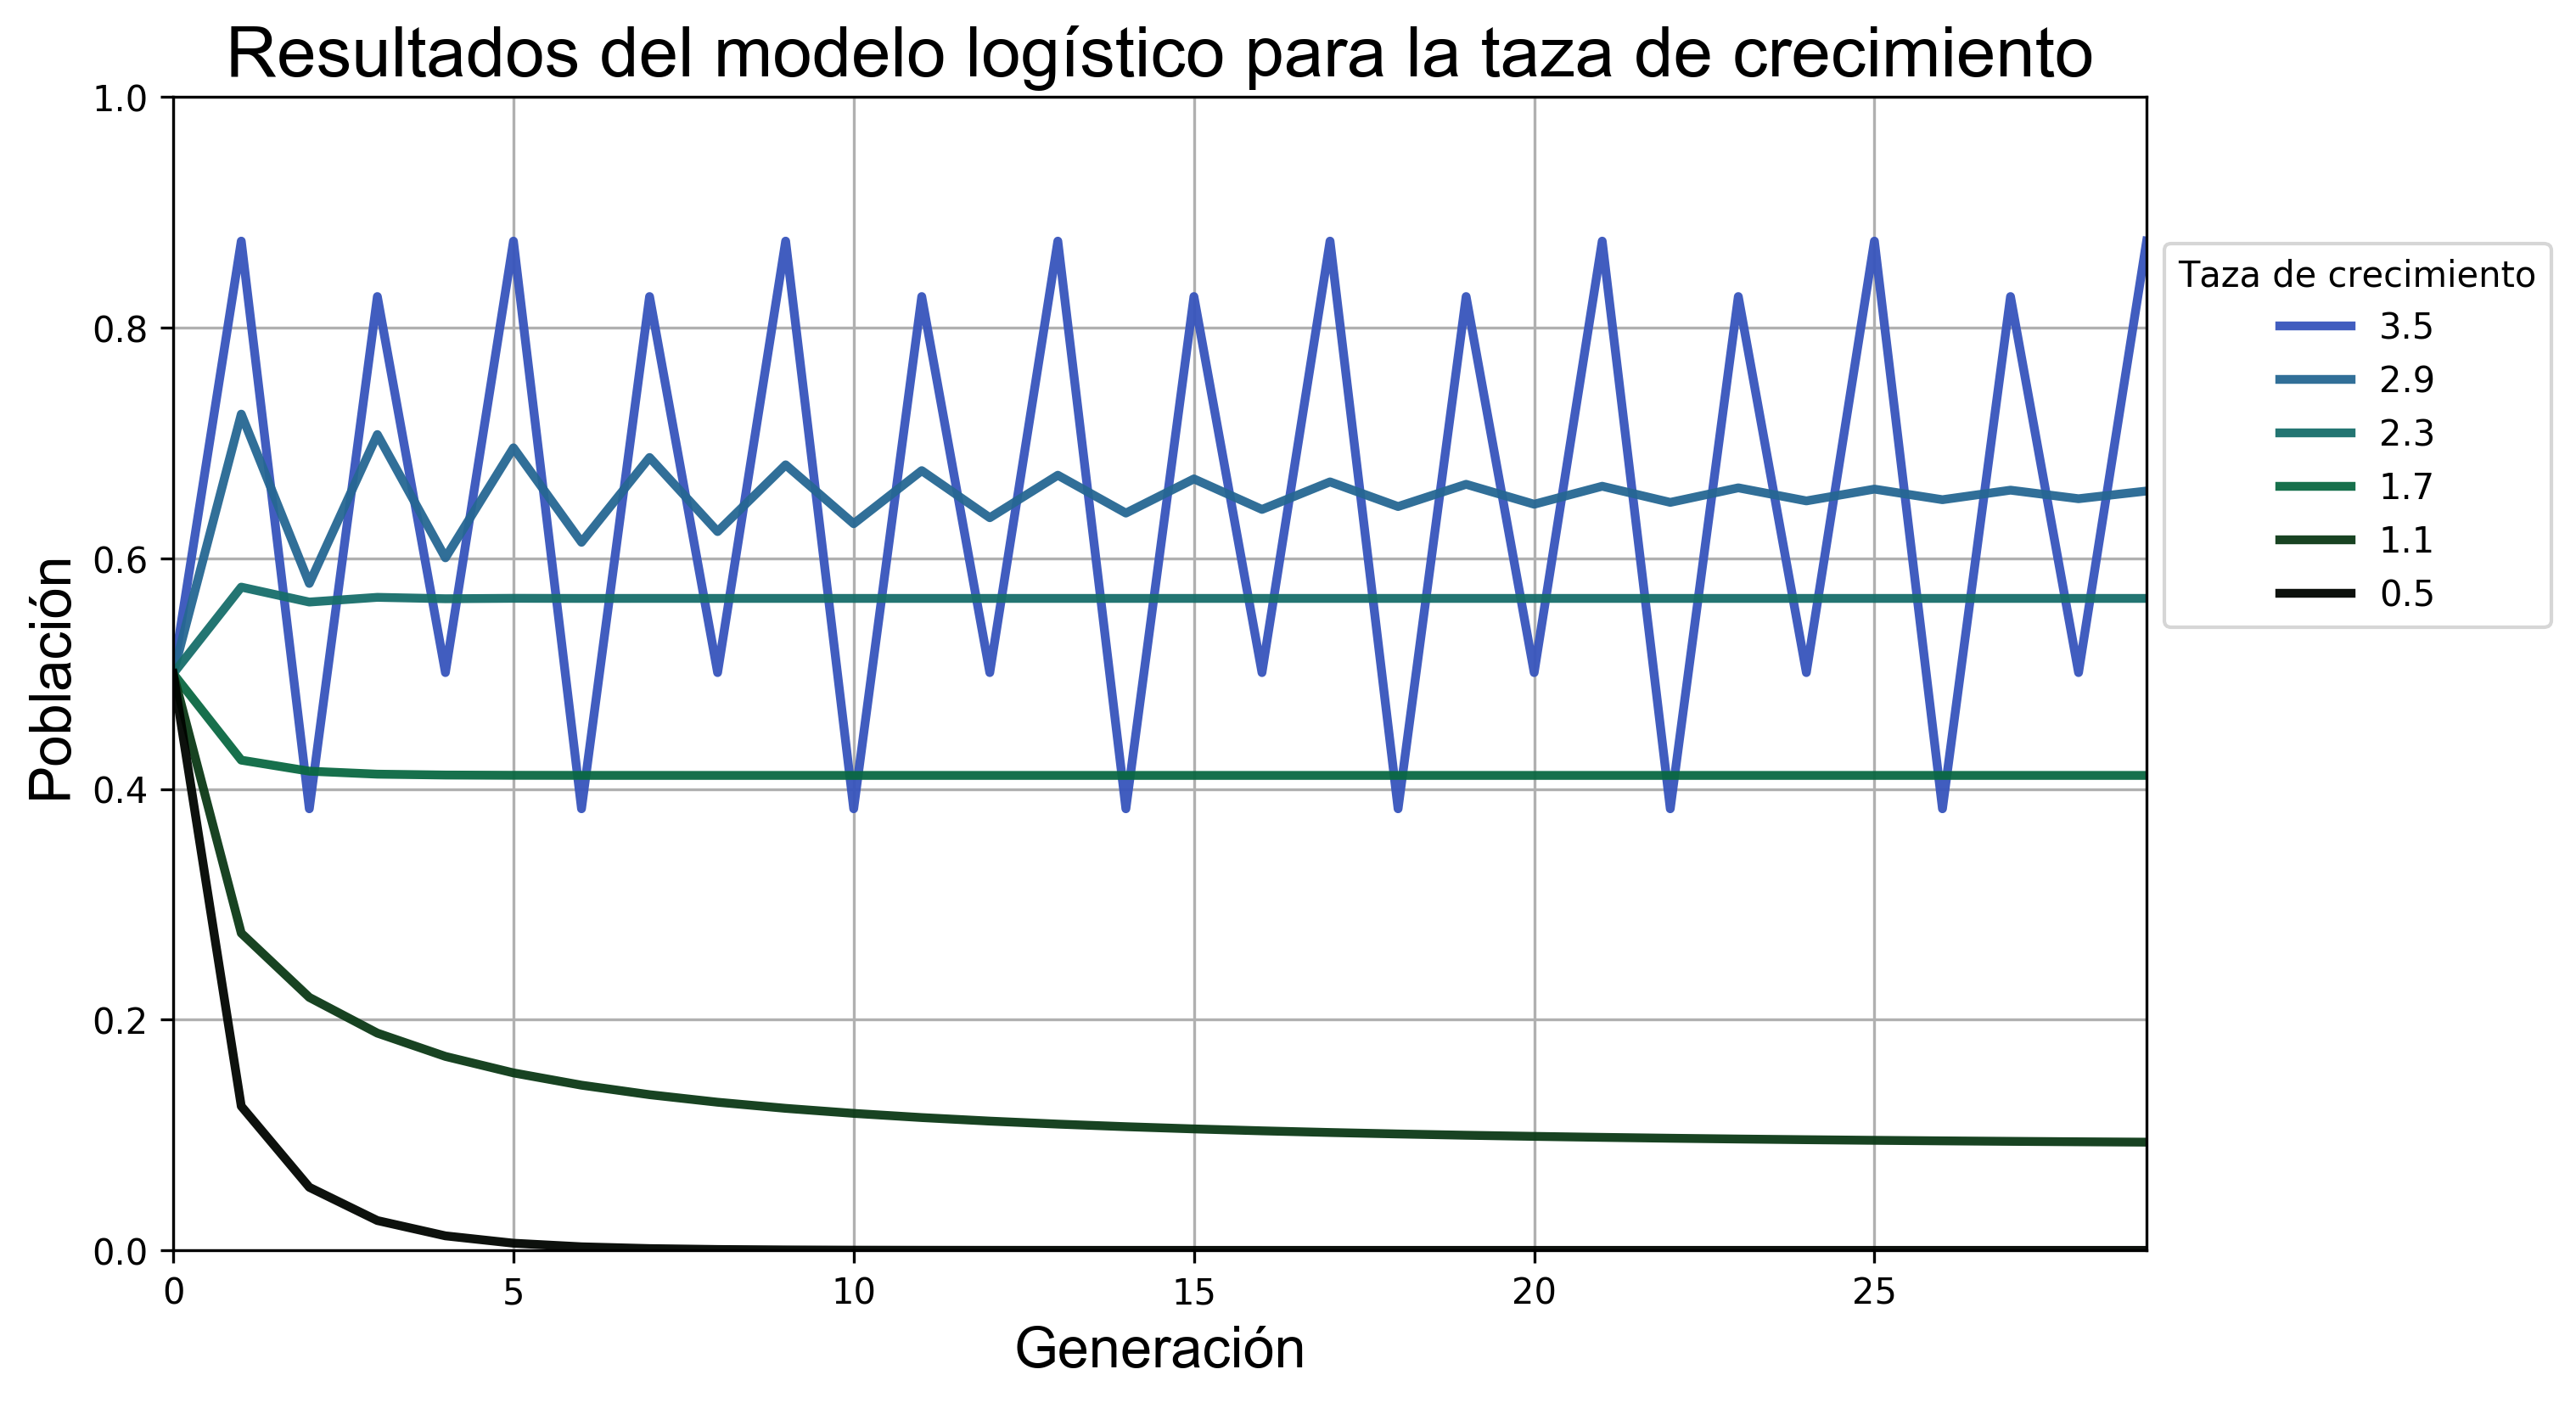
\includegraphics[scale=0.60]{logistic-map-growth-rates.png}
\end{center}

En casos como estos, en los que tomamos una gran cantidad de generaciones porque la muestra de datos es muy grande, se crean bifuraciones. Las bifuraciones son particiones en la muestra. En ellas se puede notar los cambios en la taza de crecimiento cuando la población va en aumento.\\

A continuación se presentan algunos diagramas de bifuración con dsitintos rangos de población, crecimiento y número de generaciones.

\begin{itemize}
\item Cian: 100 generaciones
\item Azul: 200 generaciones
\item Amarillo: 300 generaciones
\item Rojo: 200 generaciones
\item Verde: 500 generaciones
\end{itemize}

\vspace{1cm}

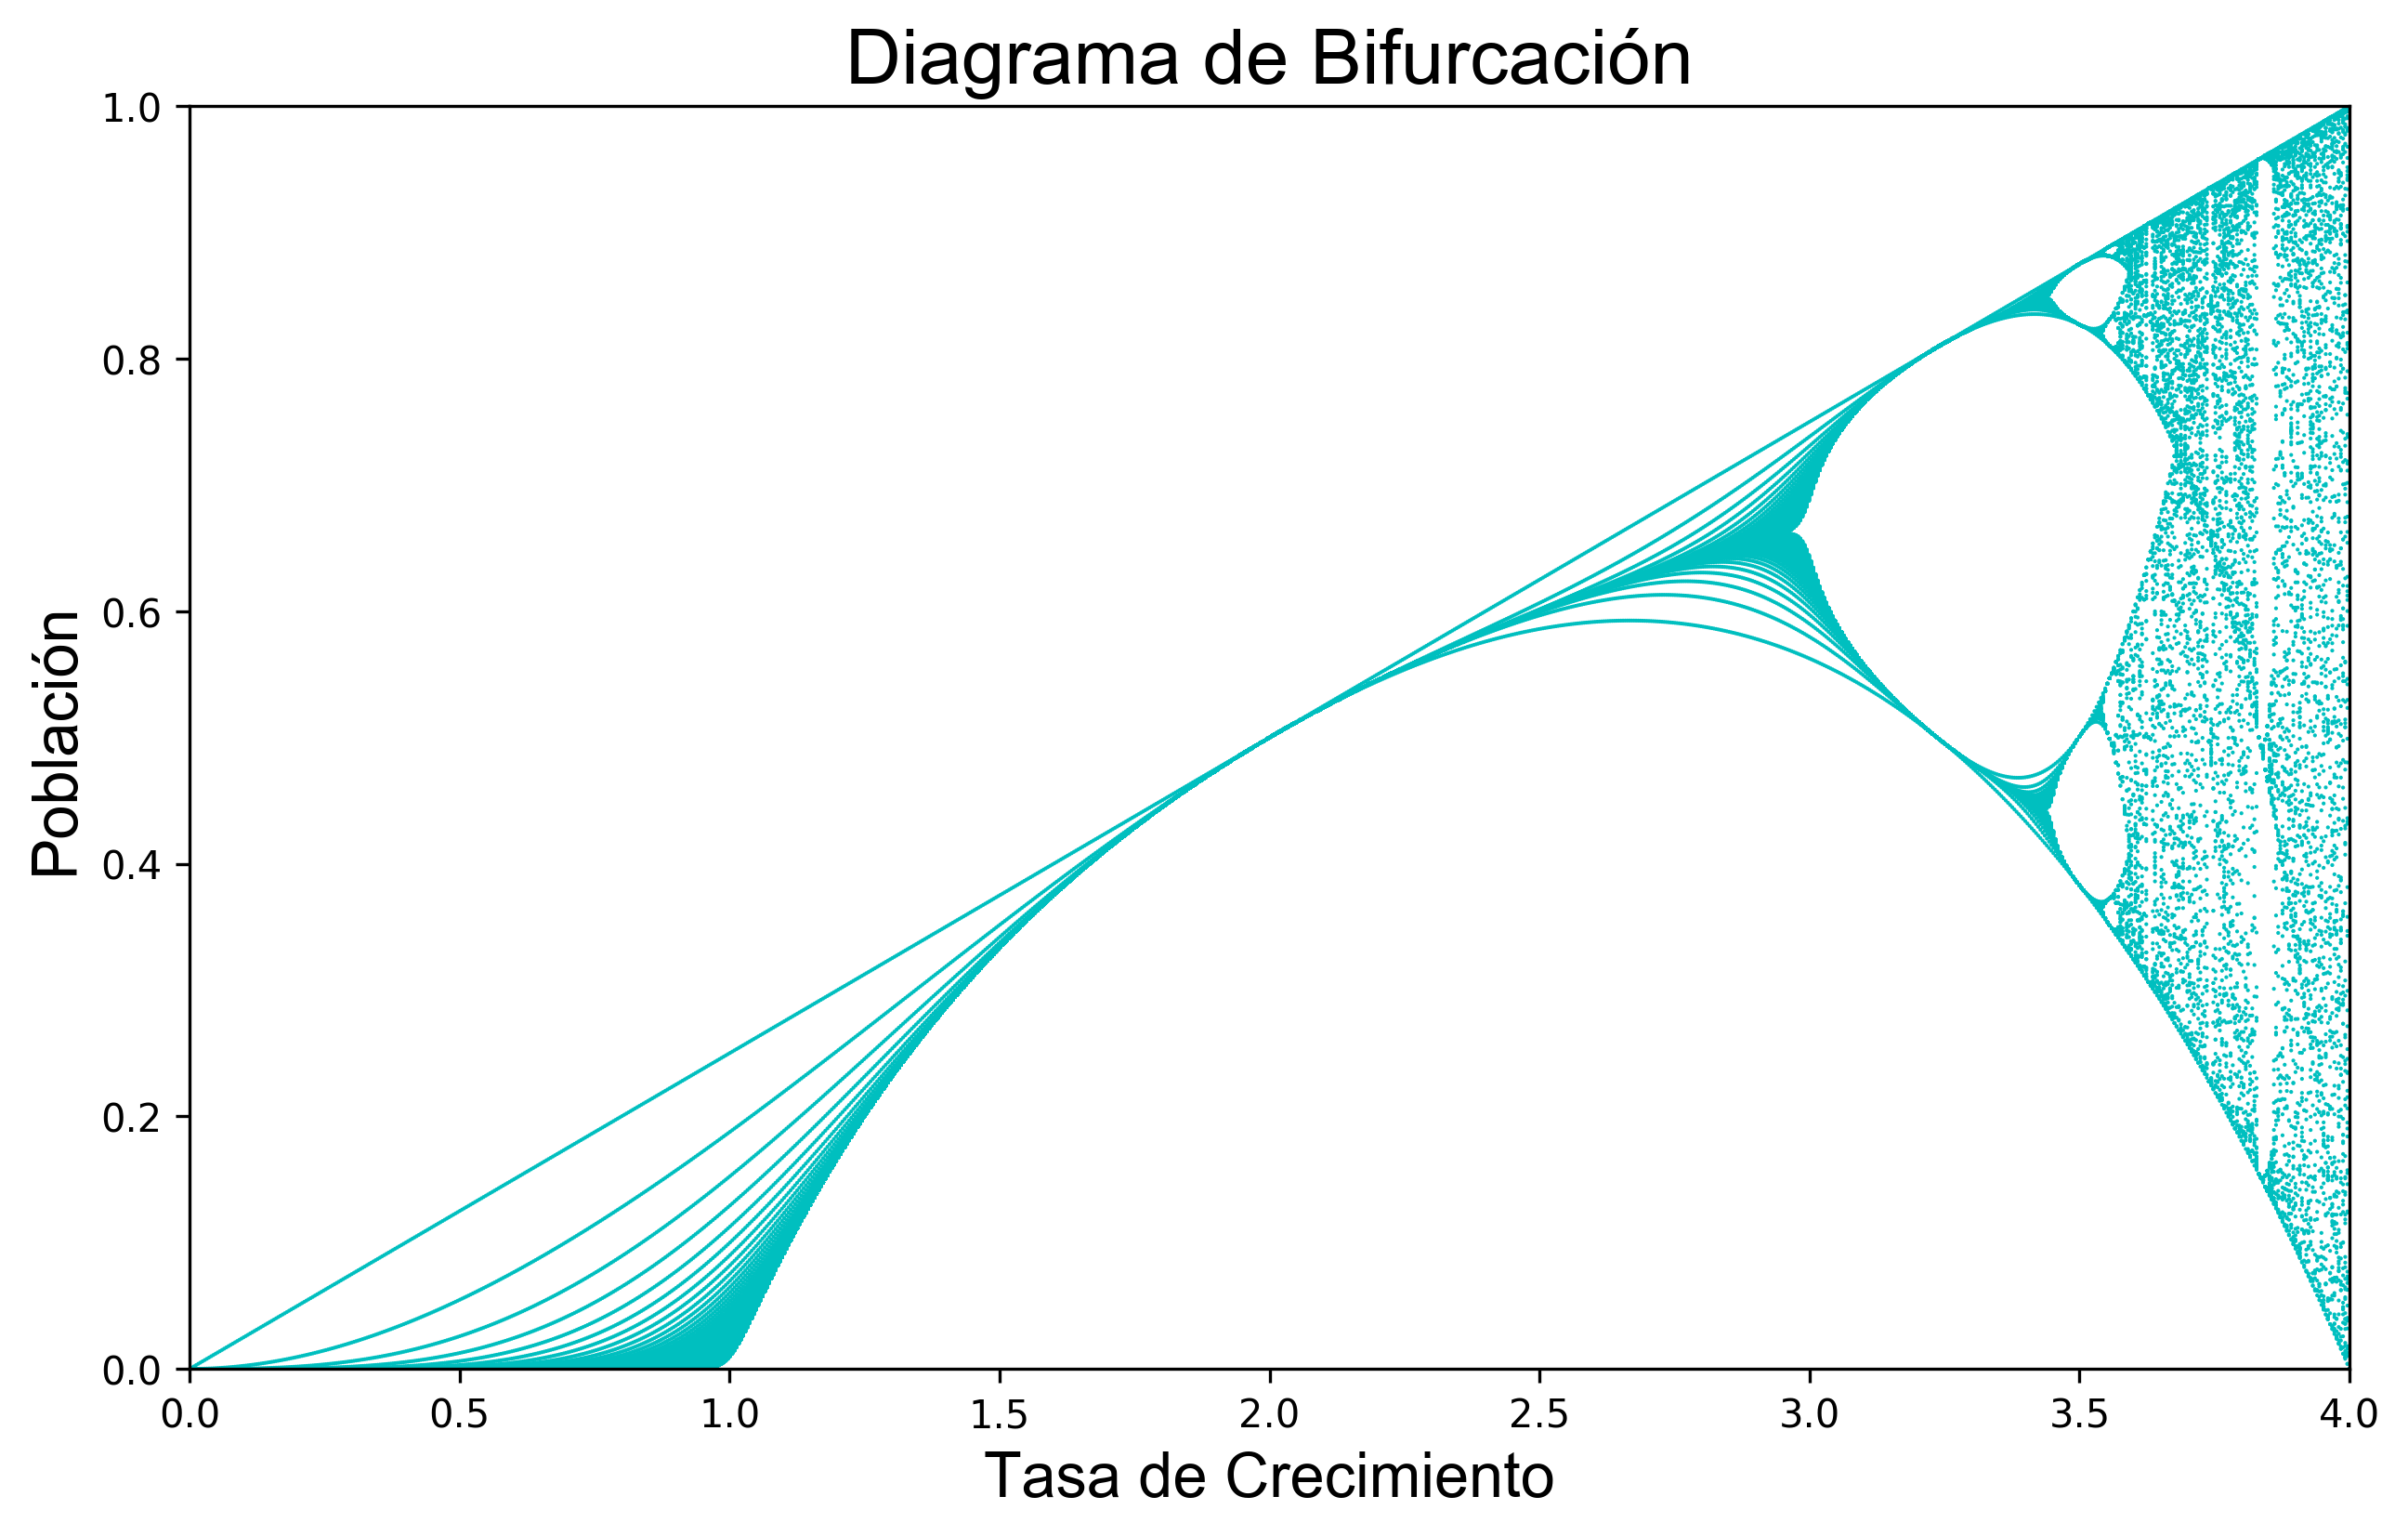
\includegraphics[scale=0.37]{logistic-map-bifurcation-0.png} \hspace{0.01cm} 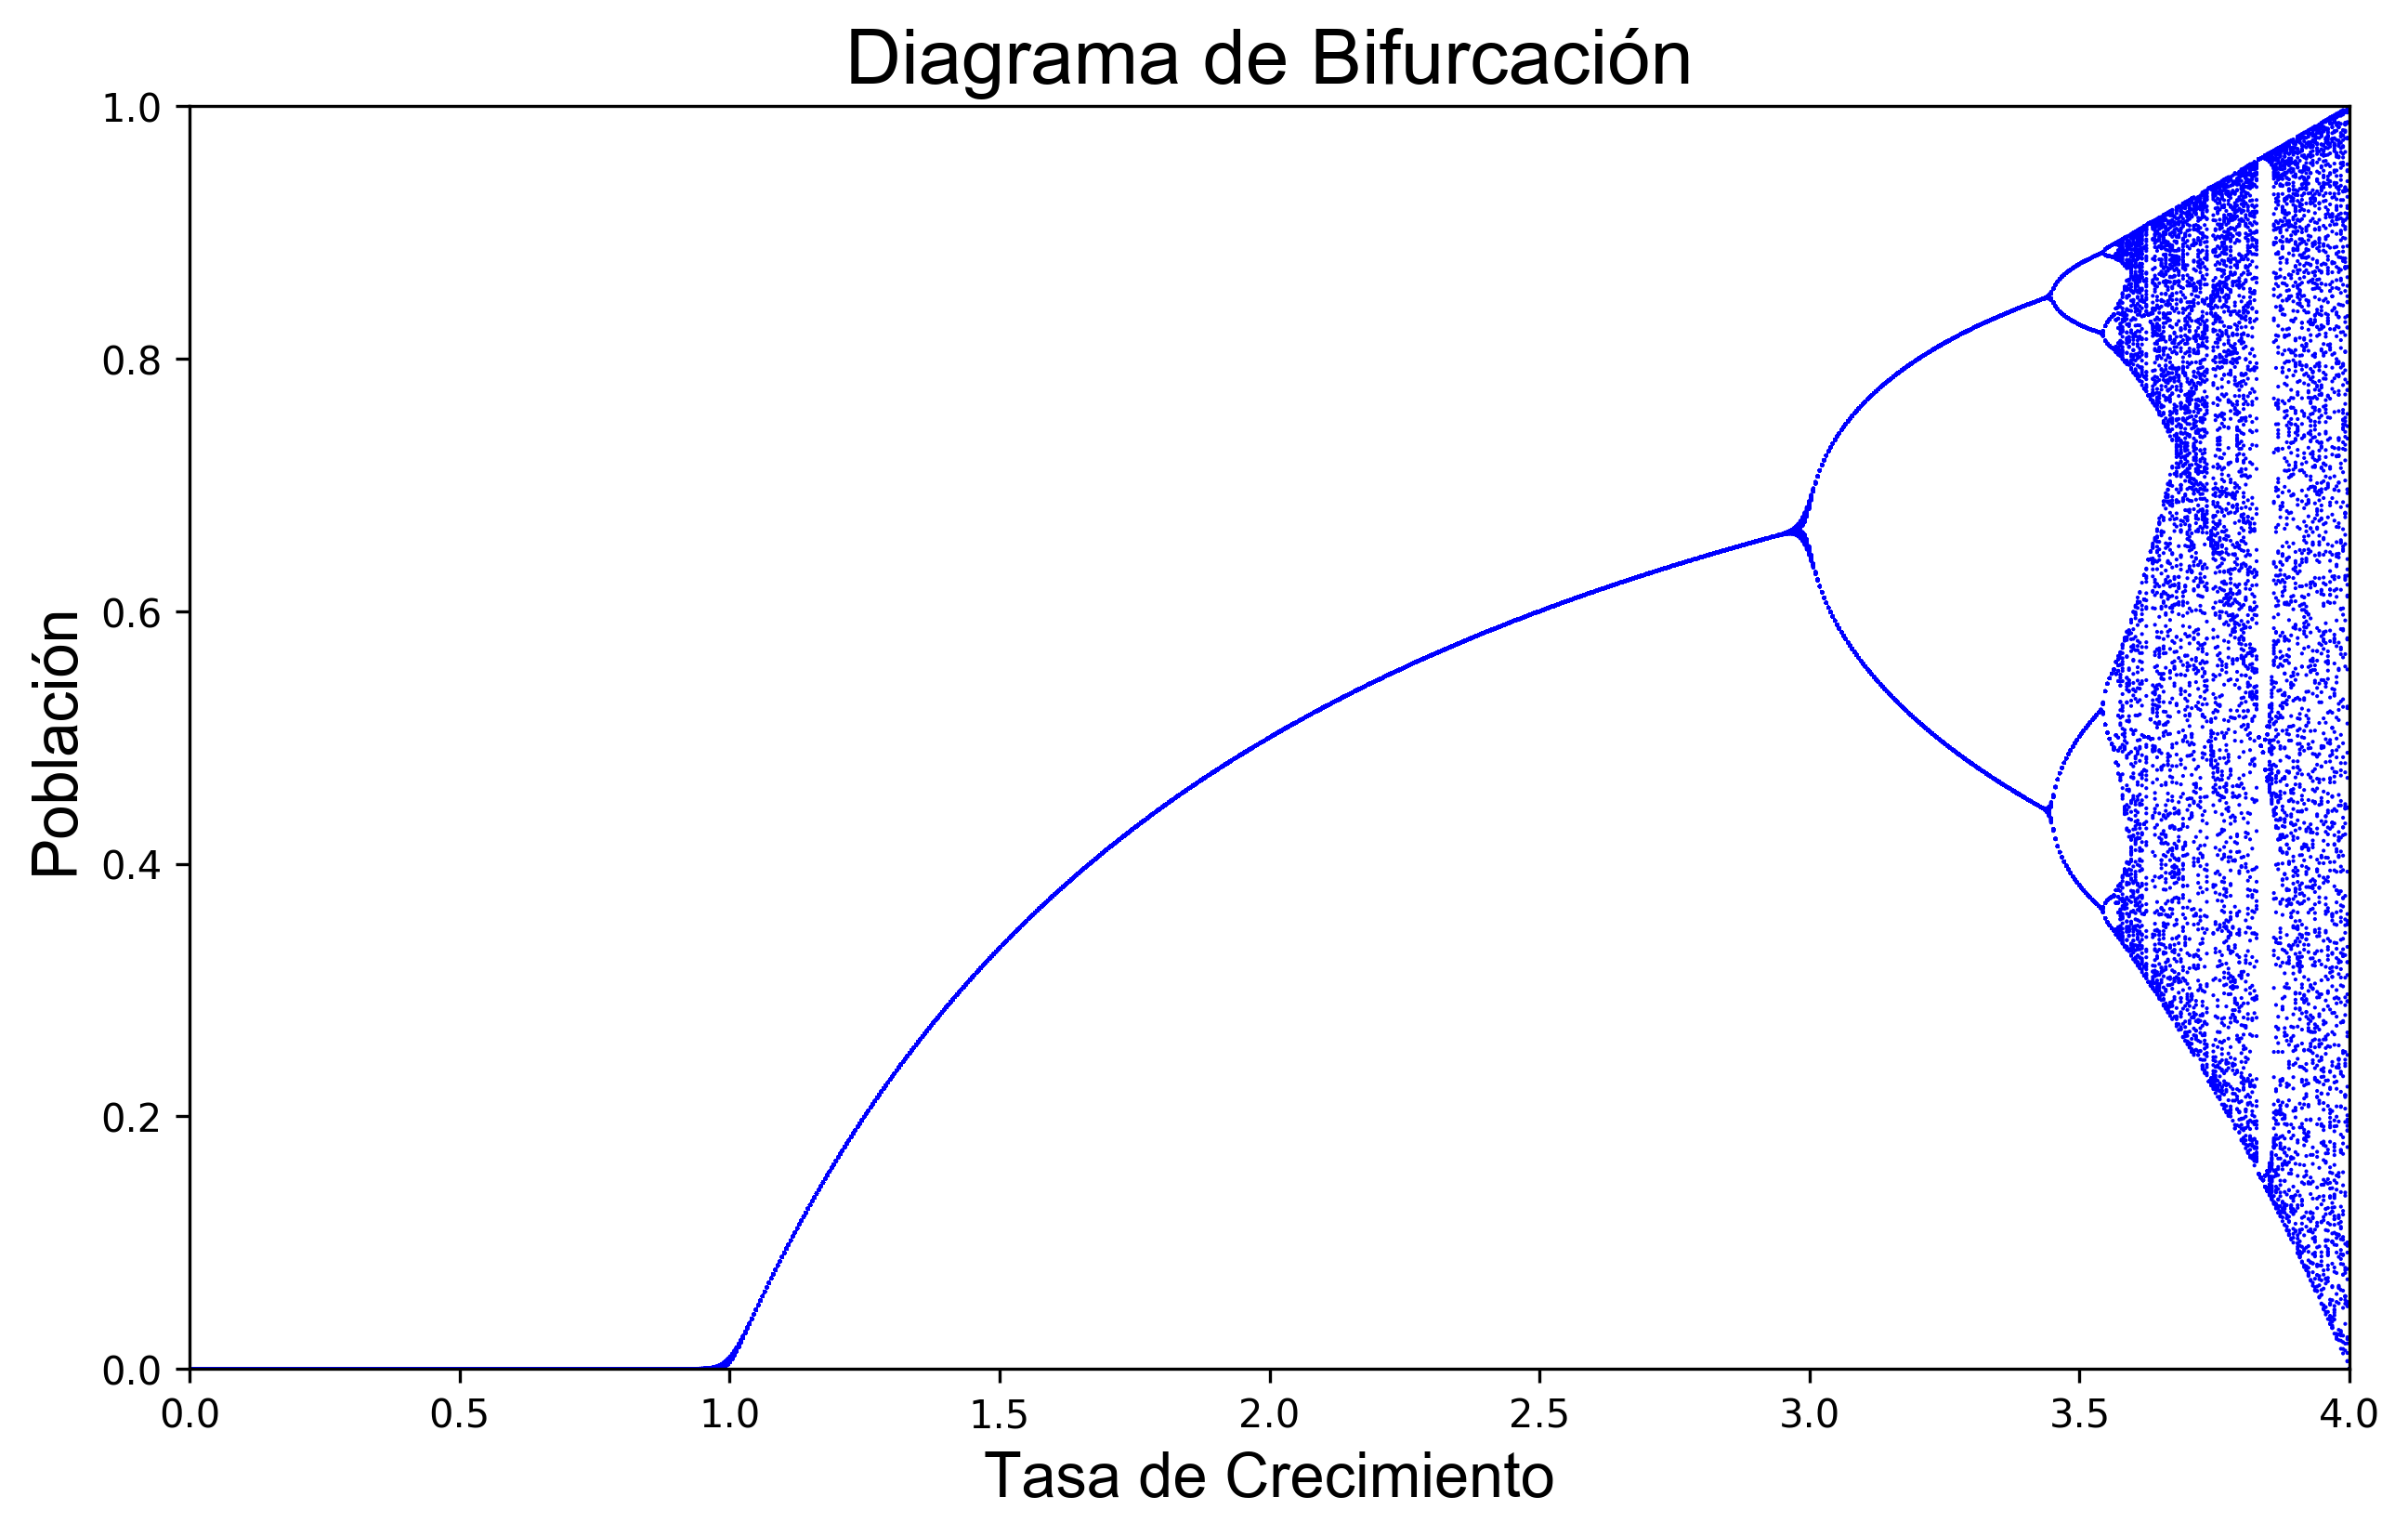
\includegraphics[scale=0.37]{logistic-map-bifurcation-1.png}

\vspace{1.2cm}

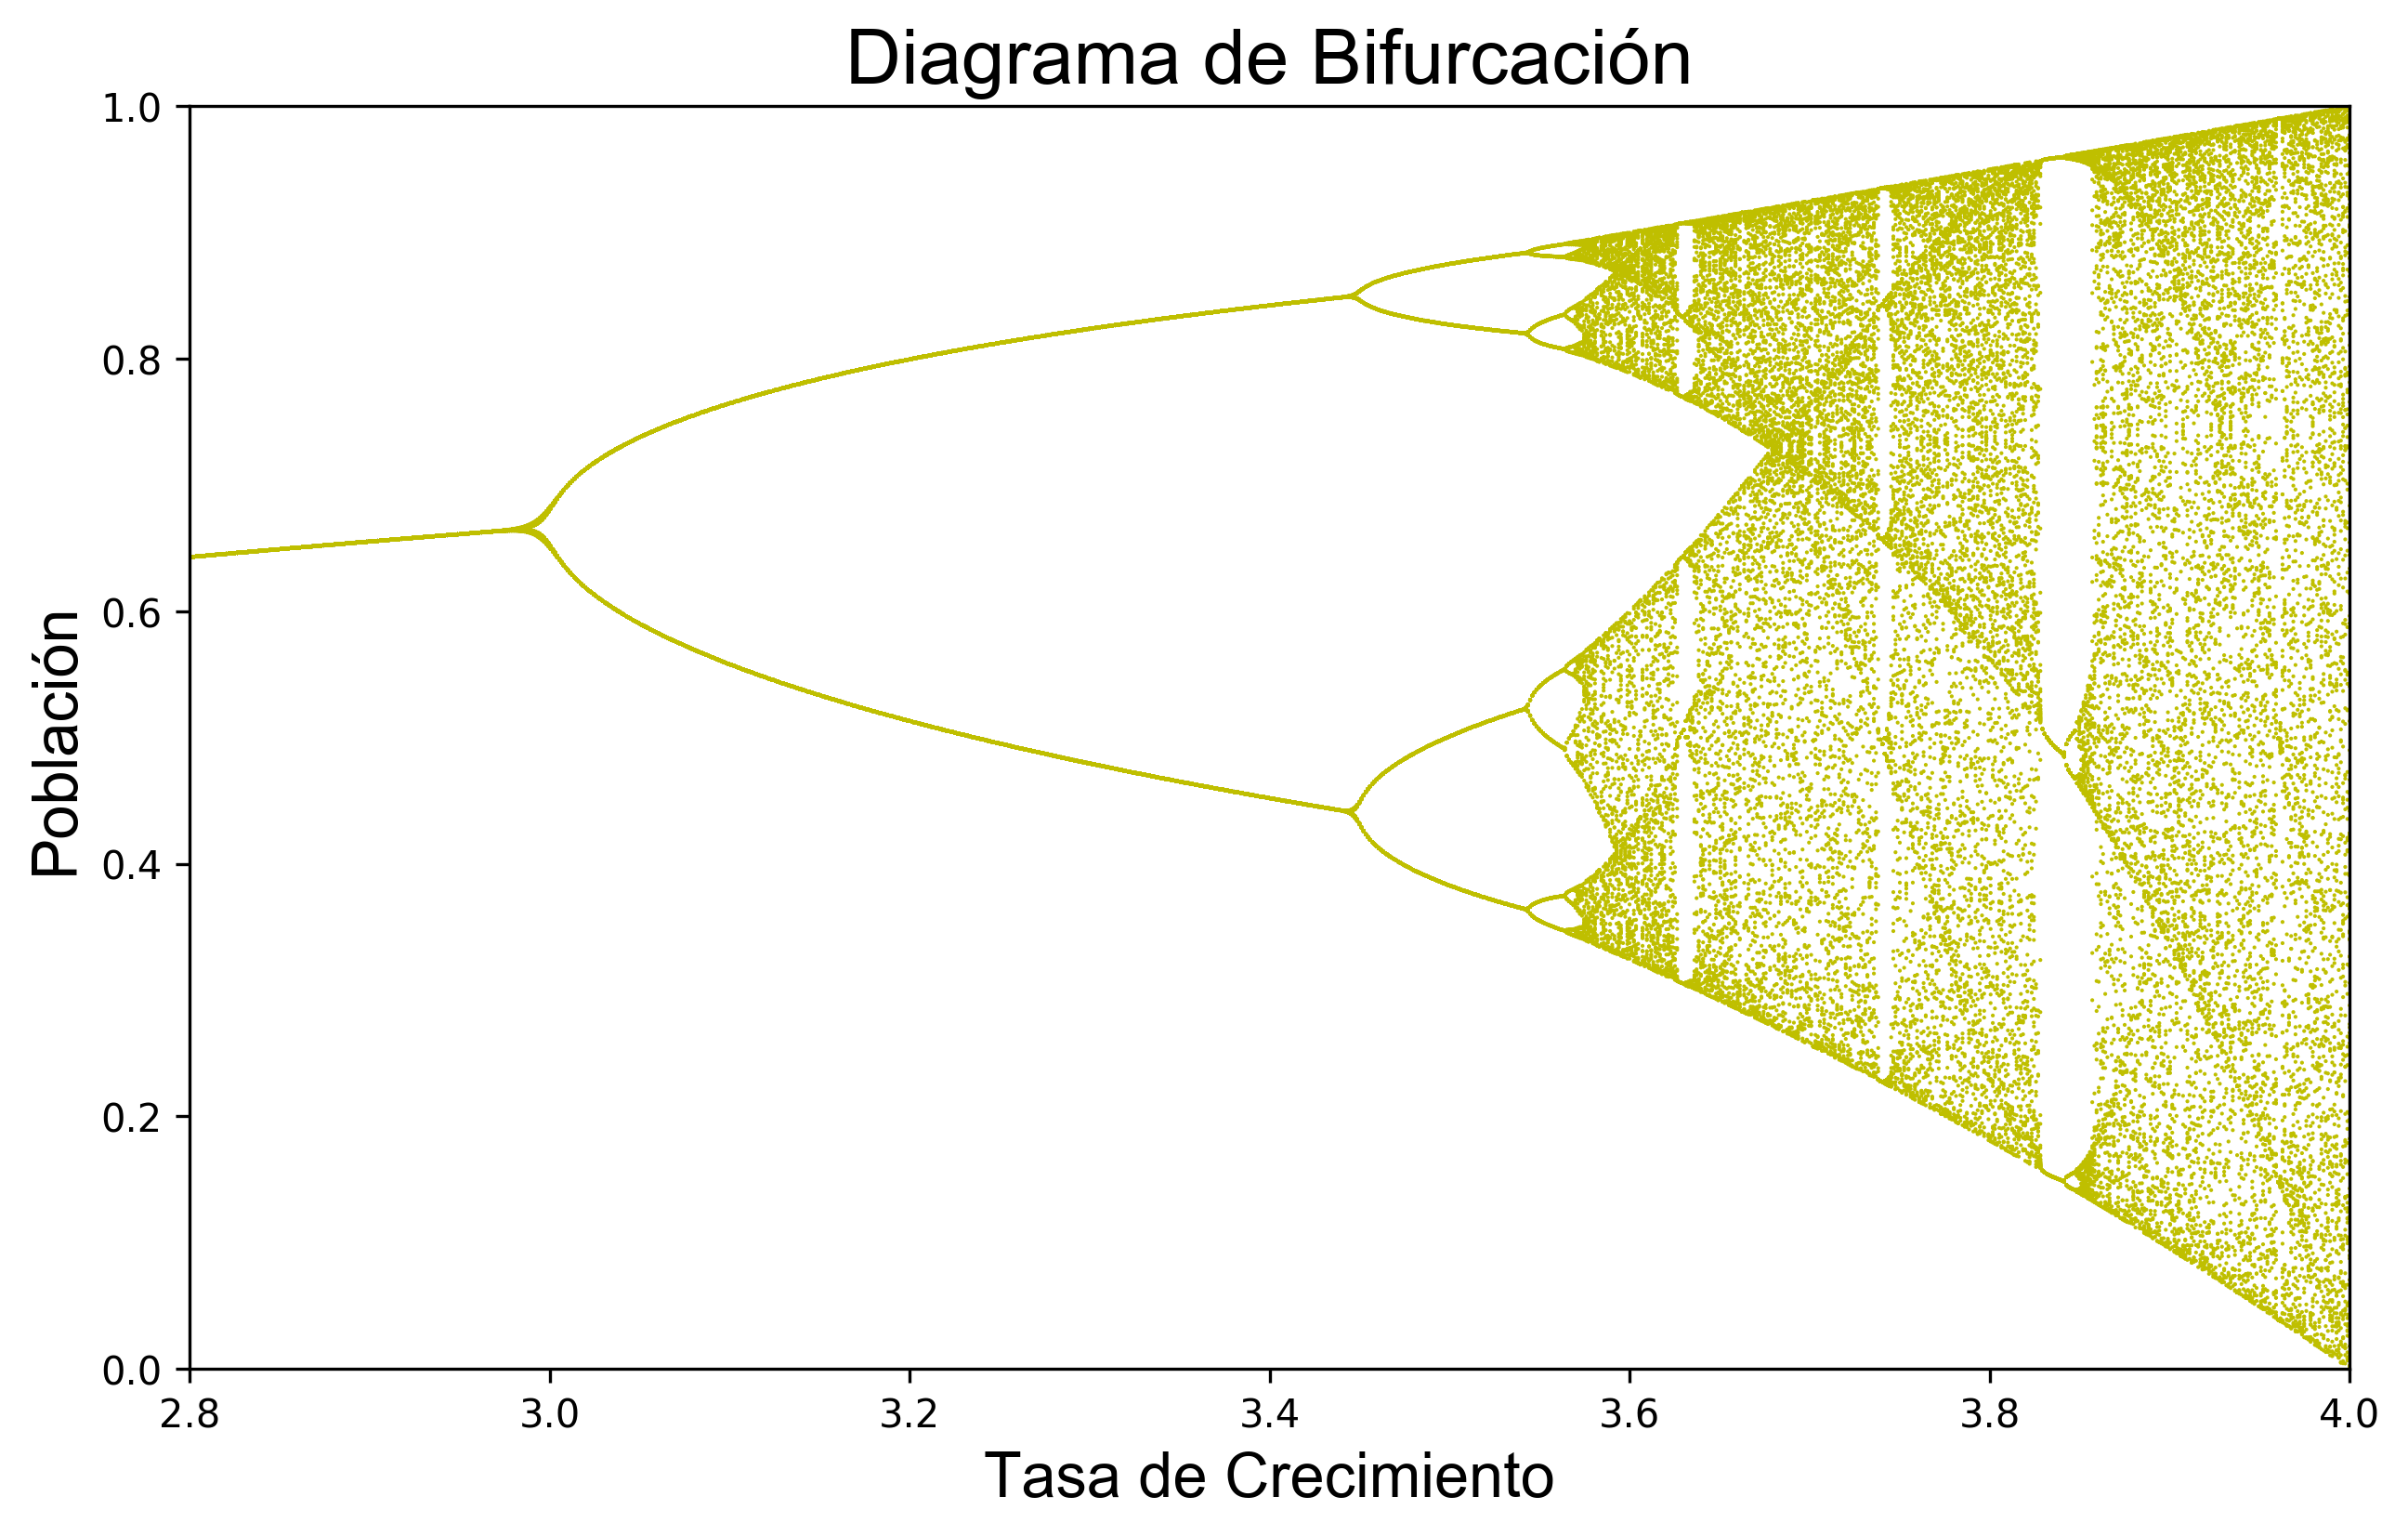
\includegraphics[scale=0.37]{logistic-map-bifurcation-2.png} \hspace{0.01cm} 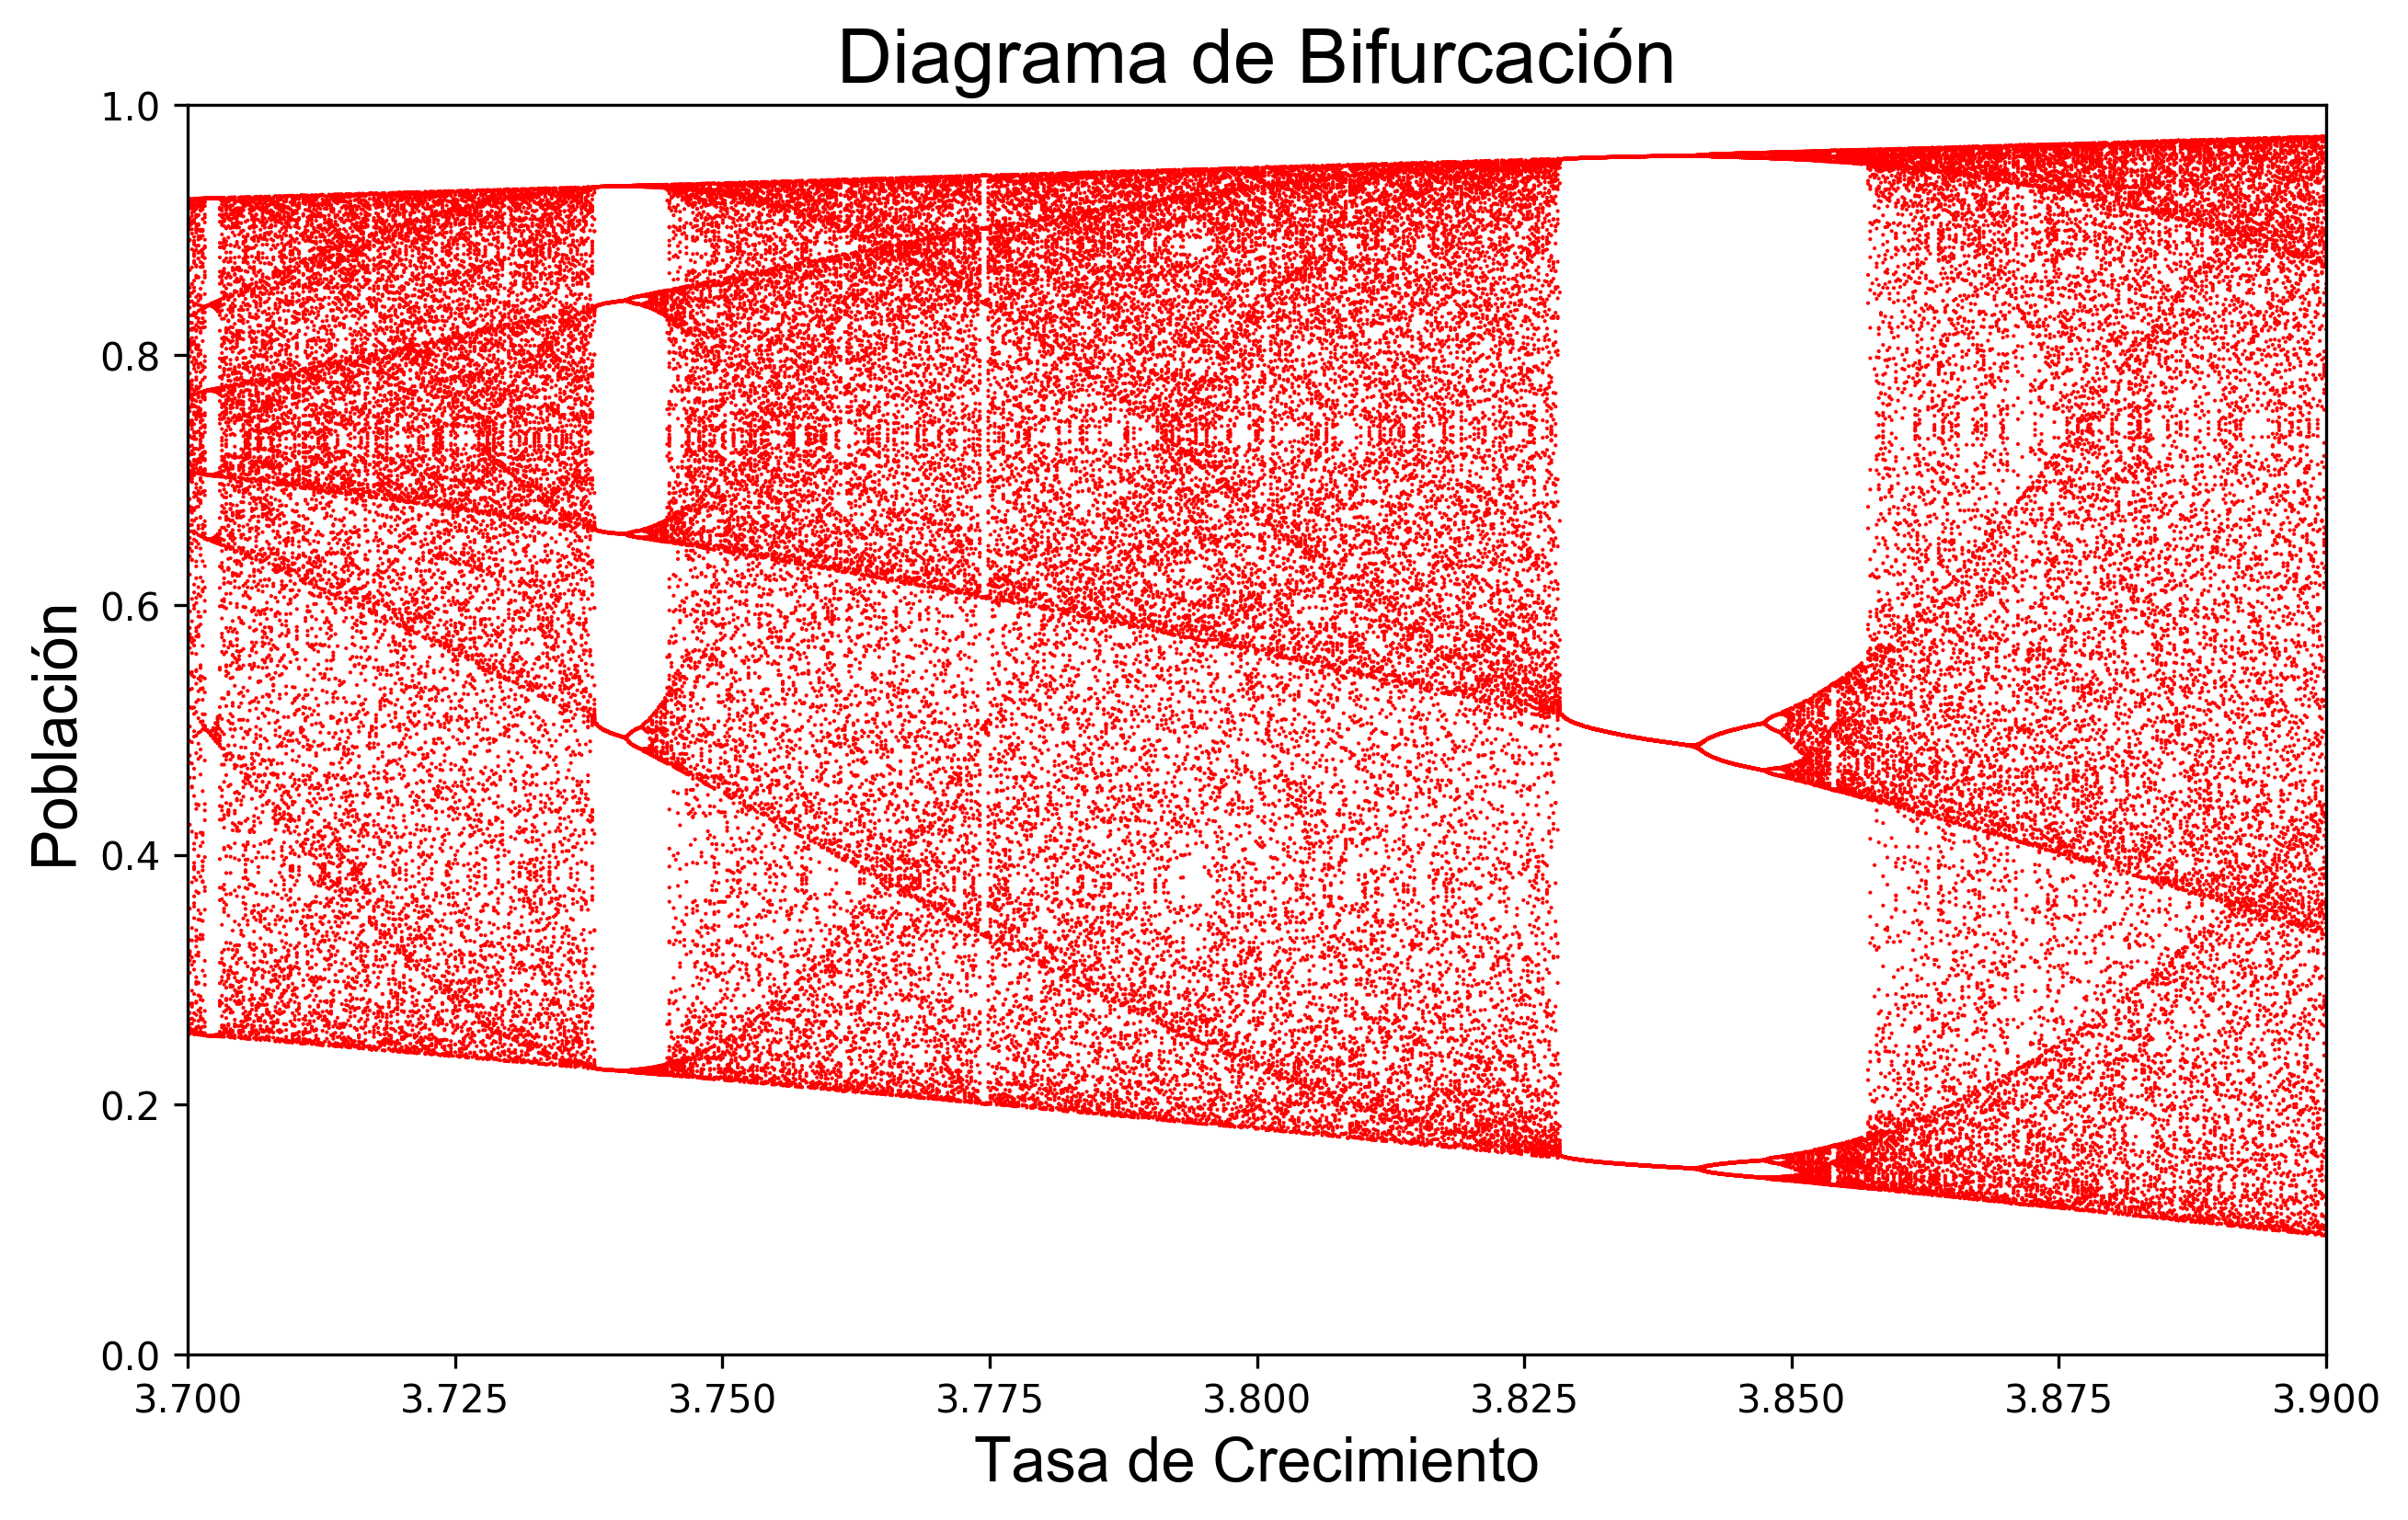
\includegraphics[scale=0.37]{logistic-map-bifurcation-3.png}


\begin{center}
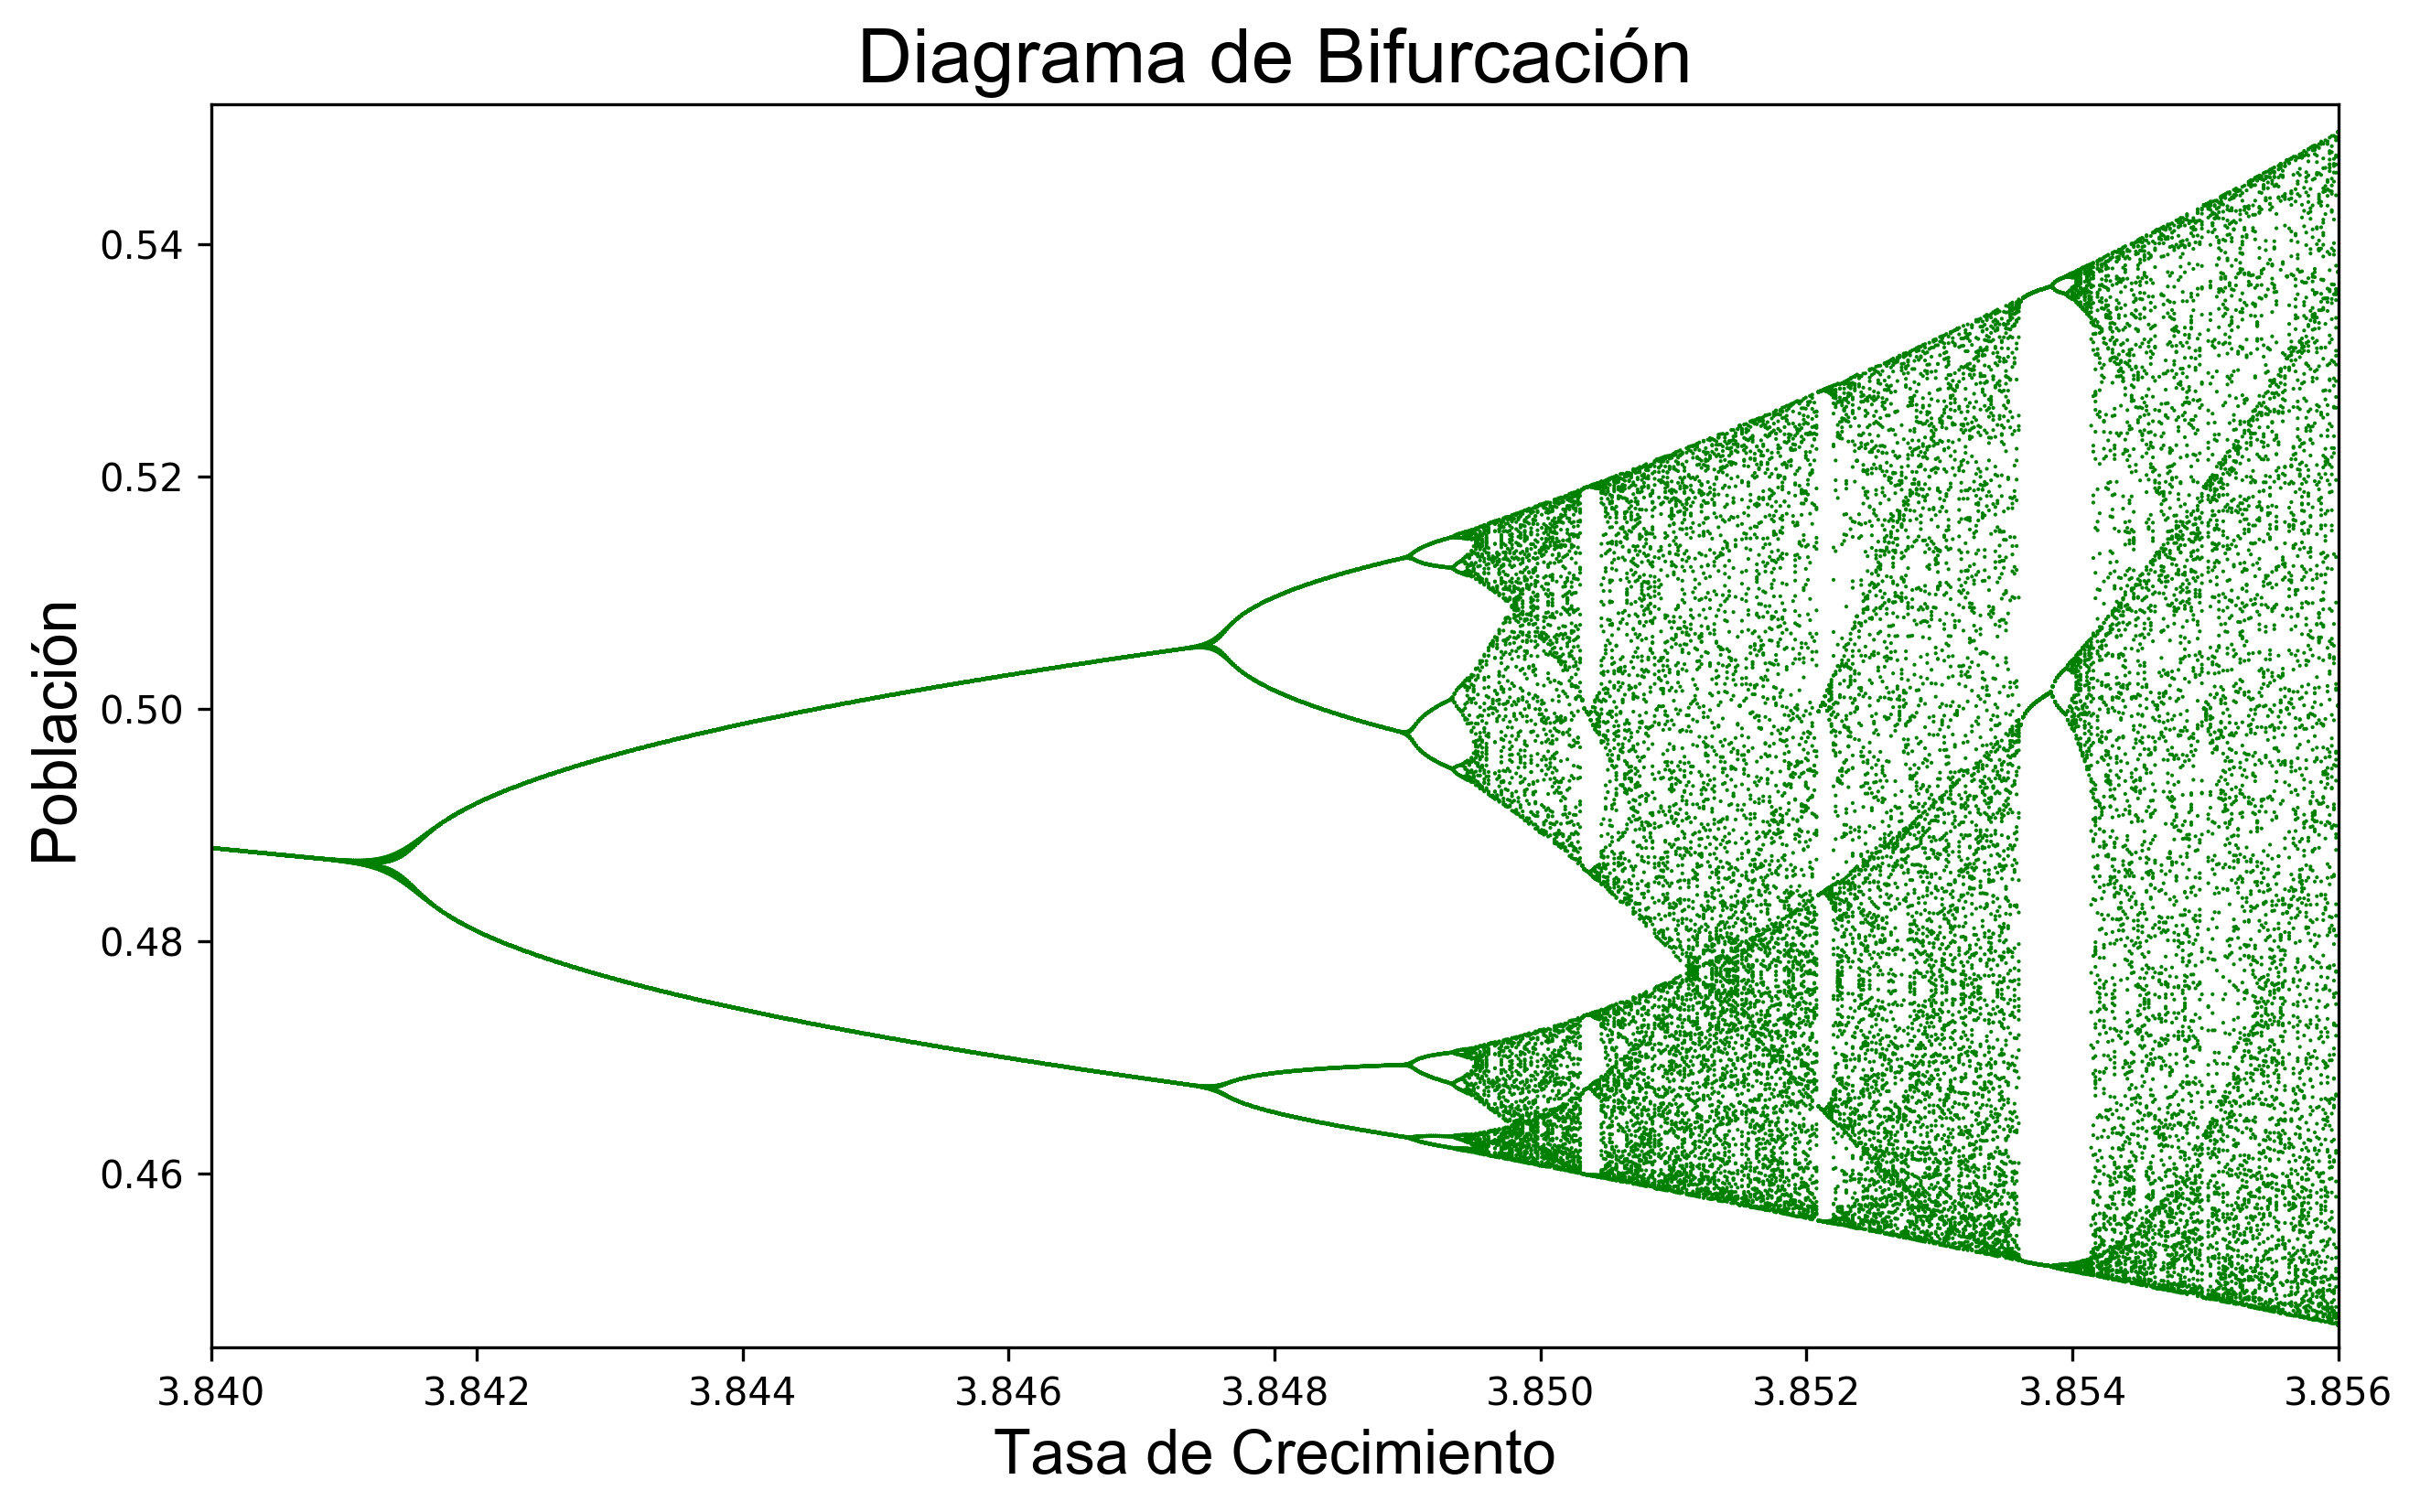
\includegraphics[scale=0.50]{logistic-map-bifurcation-4.png}
\end{center}

\vspace{1.5cm}

Otra cosa que se puede analizar mediantes las gráficas posibles de realizar en python es el comportamiento de la población segun la generación. Para esto nos enfocamos en una muestra con una taza de crecimiento de 3.9 y 3.0001, en las cuales podemos observar condiciones iniciales muy similares, pero que al final se vuelven muy distintas.\\ 

\vspace{0.5cm}

\begin{center}
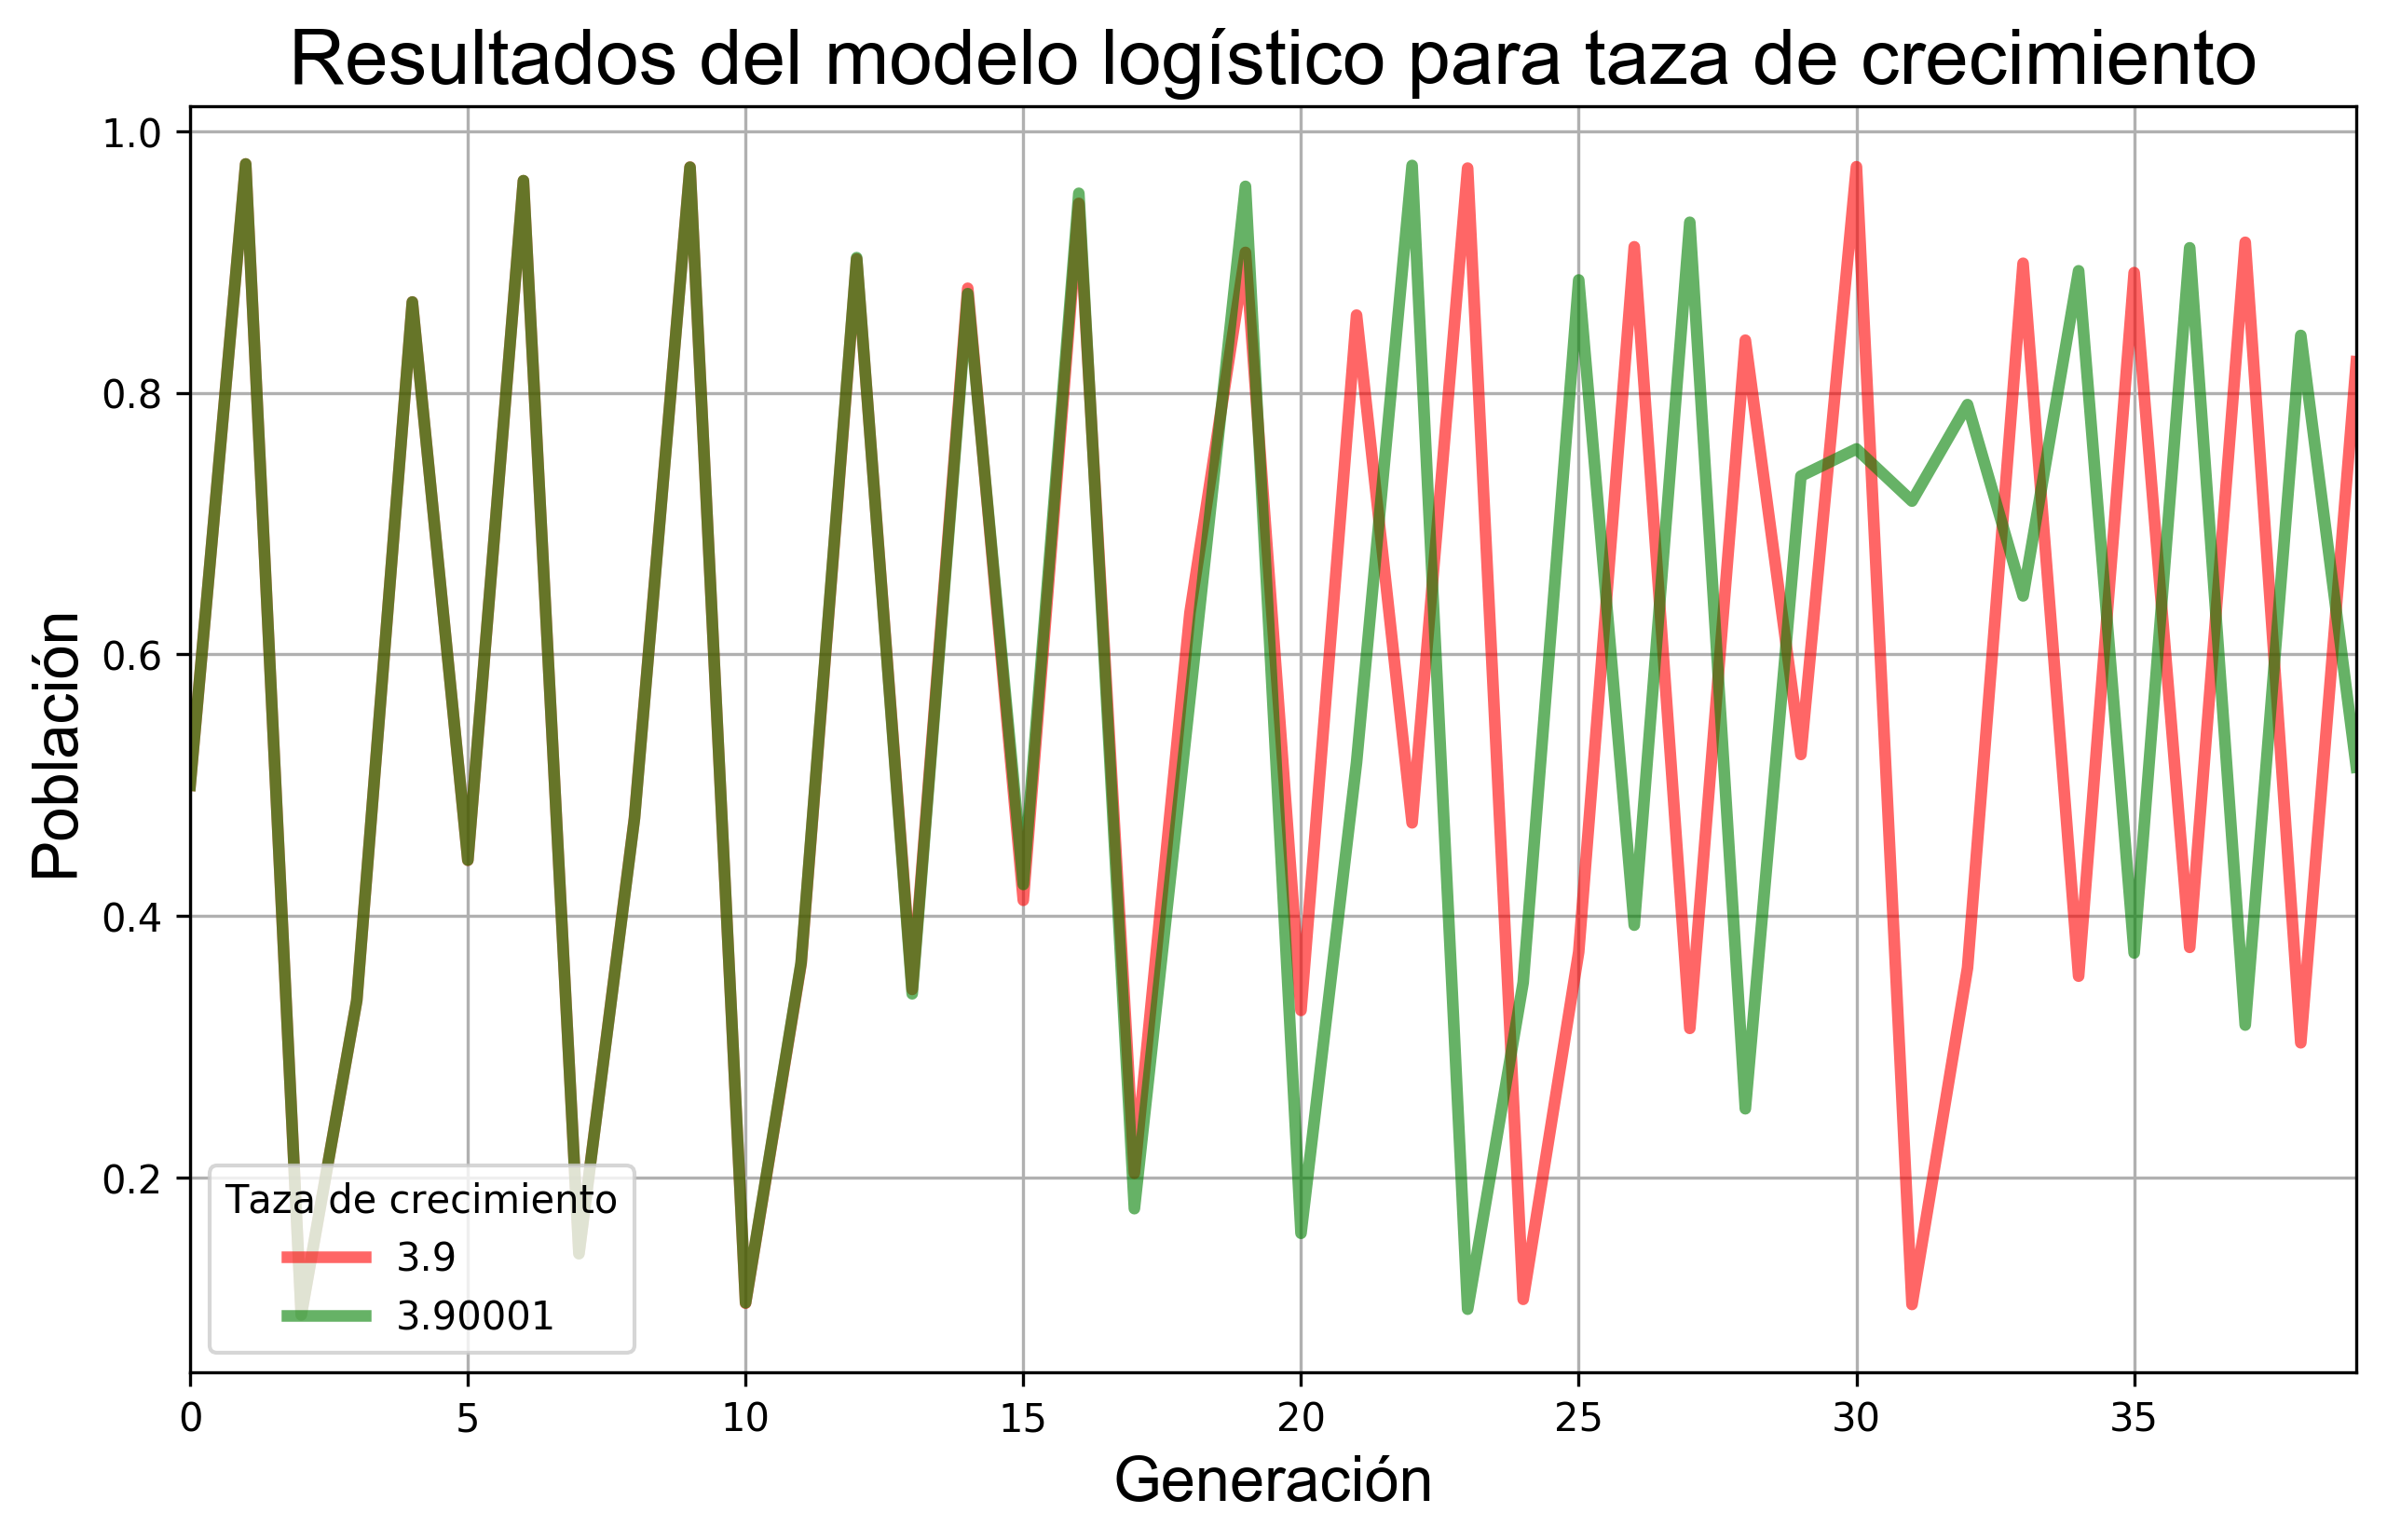
\includegraphics[scale=0.60]{logistic-map-parameter-sensitivity.png}
\end{center}

\vspace{1cm}

A continuación se ilustra otro ejemplo en el qu tenemos la misma situación anterior, pero con otras tazas de crecimiento.\\

\vspace{0.2cm}

\begin{center}
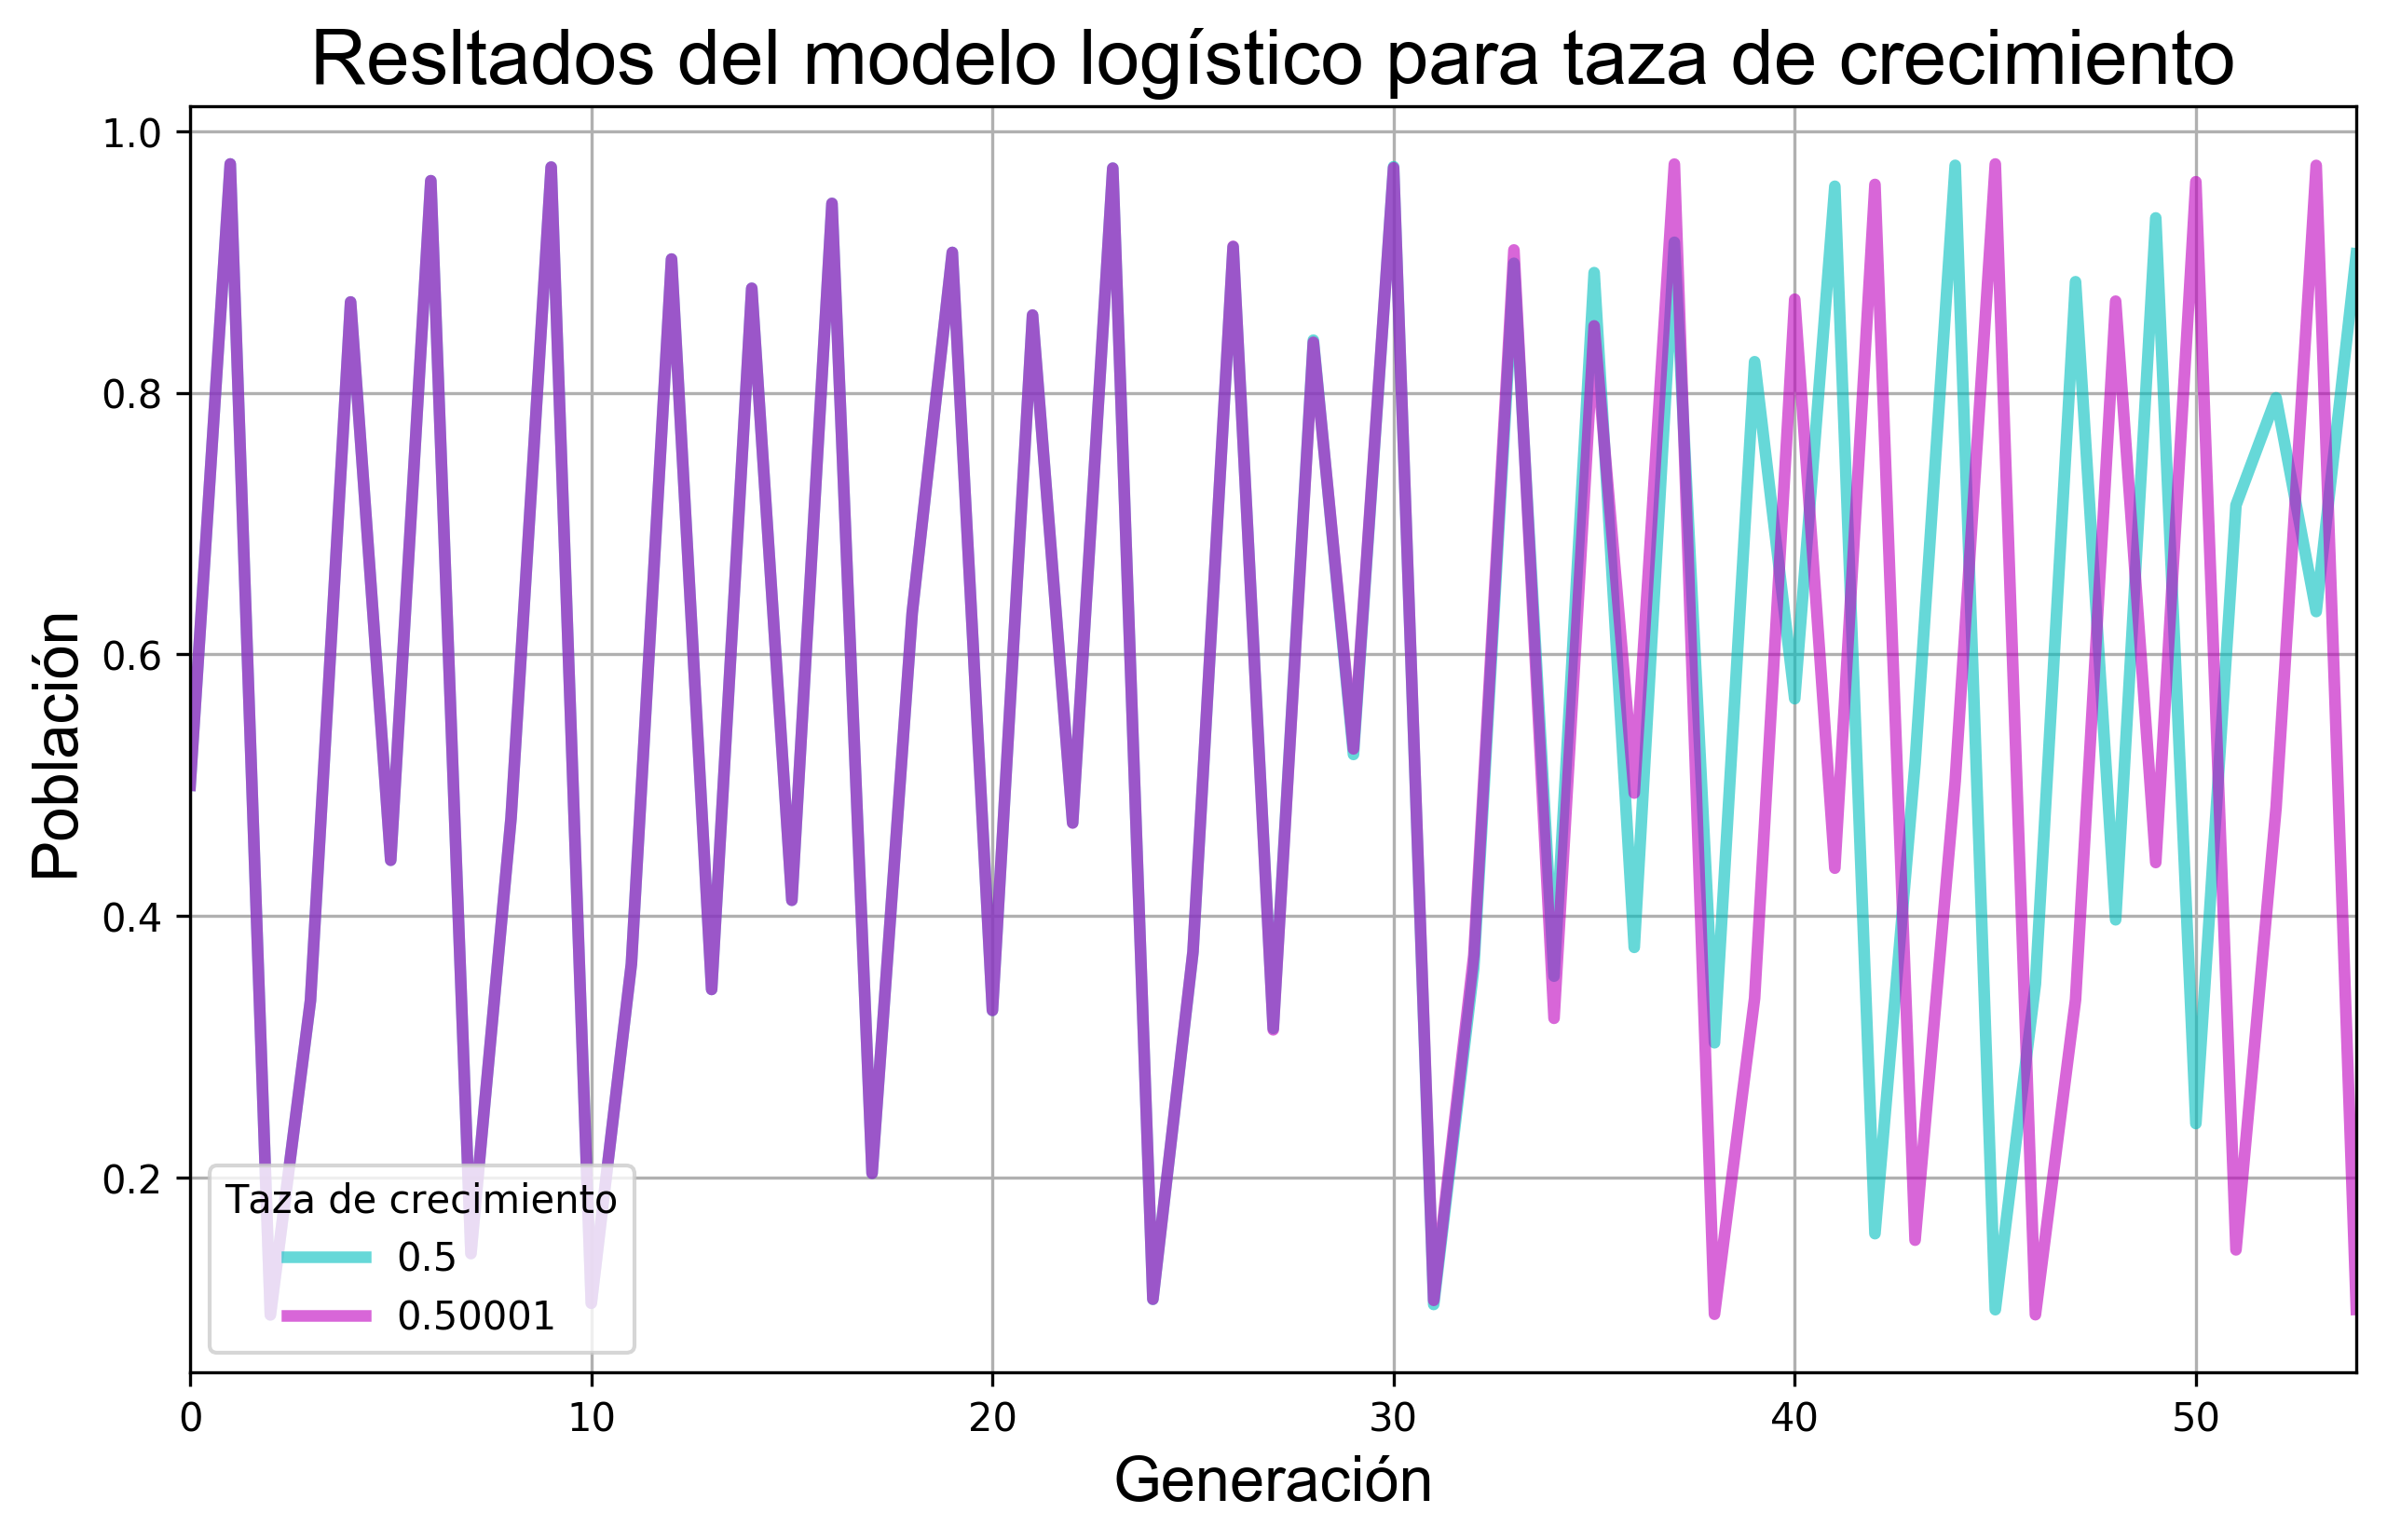
\includegraphics[scale=0.60]{logistic-map-initial-conditions.png}
\end{center}

\vspace{0.5cm}

Sin embargo, podemos notar que el sistema no es completamente caótico, pues hay ciertas tazas de crecimiento en  las que no sucede lo anterior. Un ejemplo es la taza de crecomiento de 0.5 y 0.50001.\\ 

\vspace{0.2cm}

\begin{center}
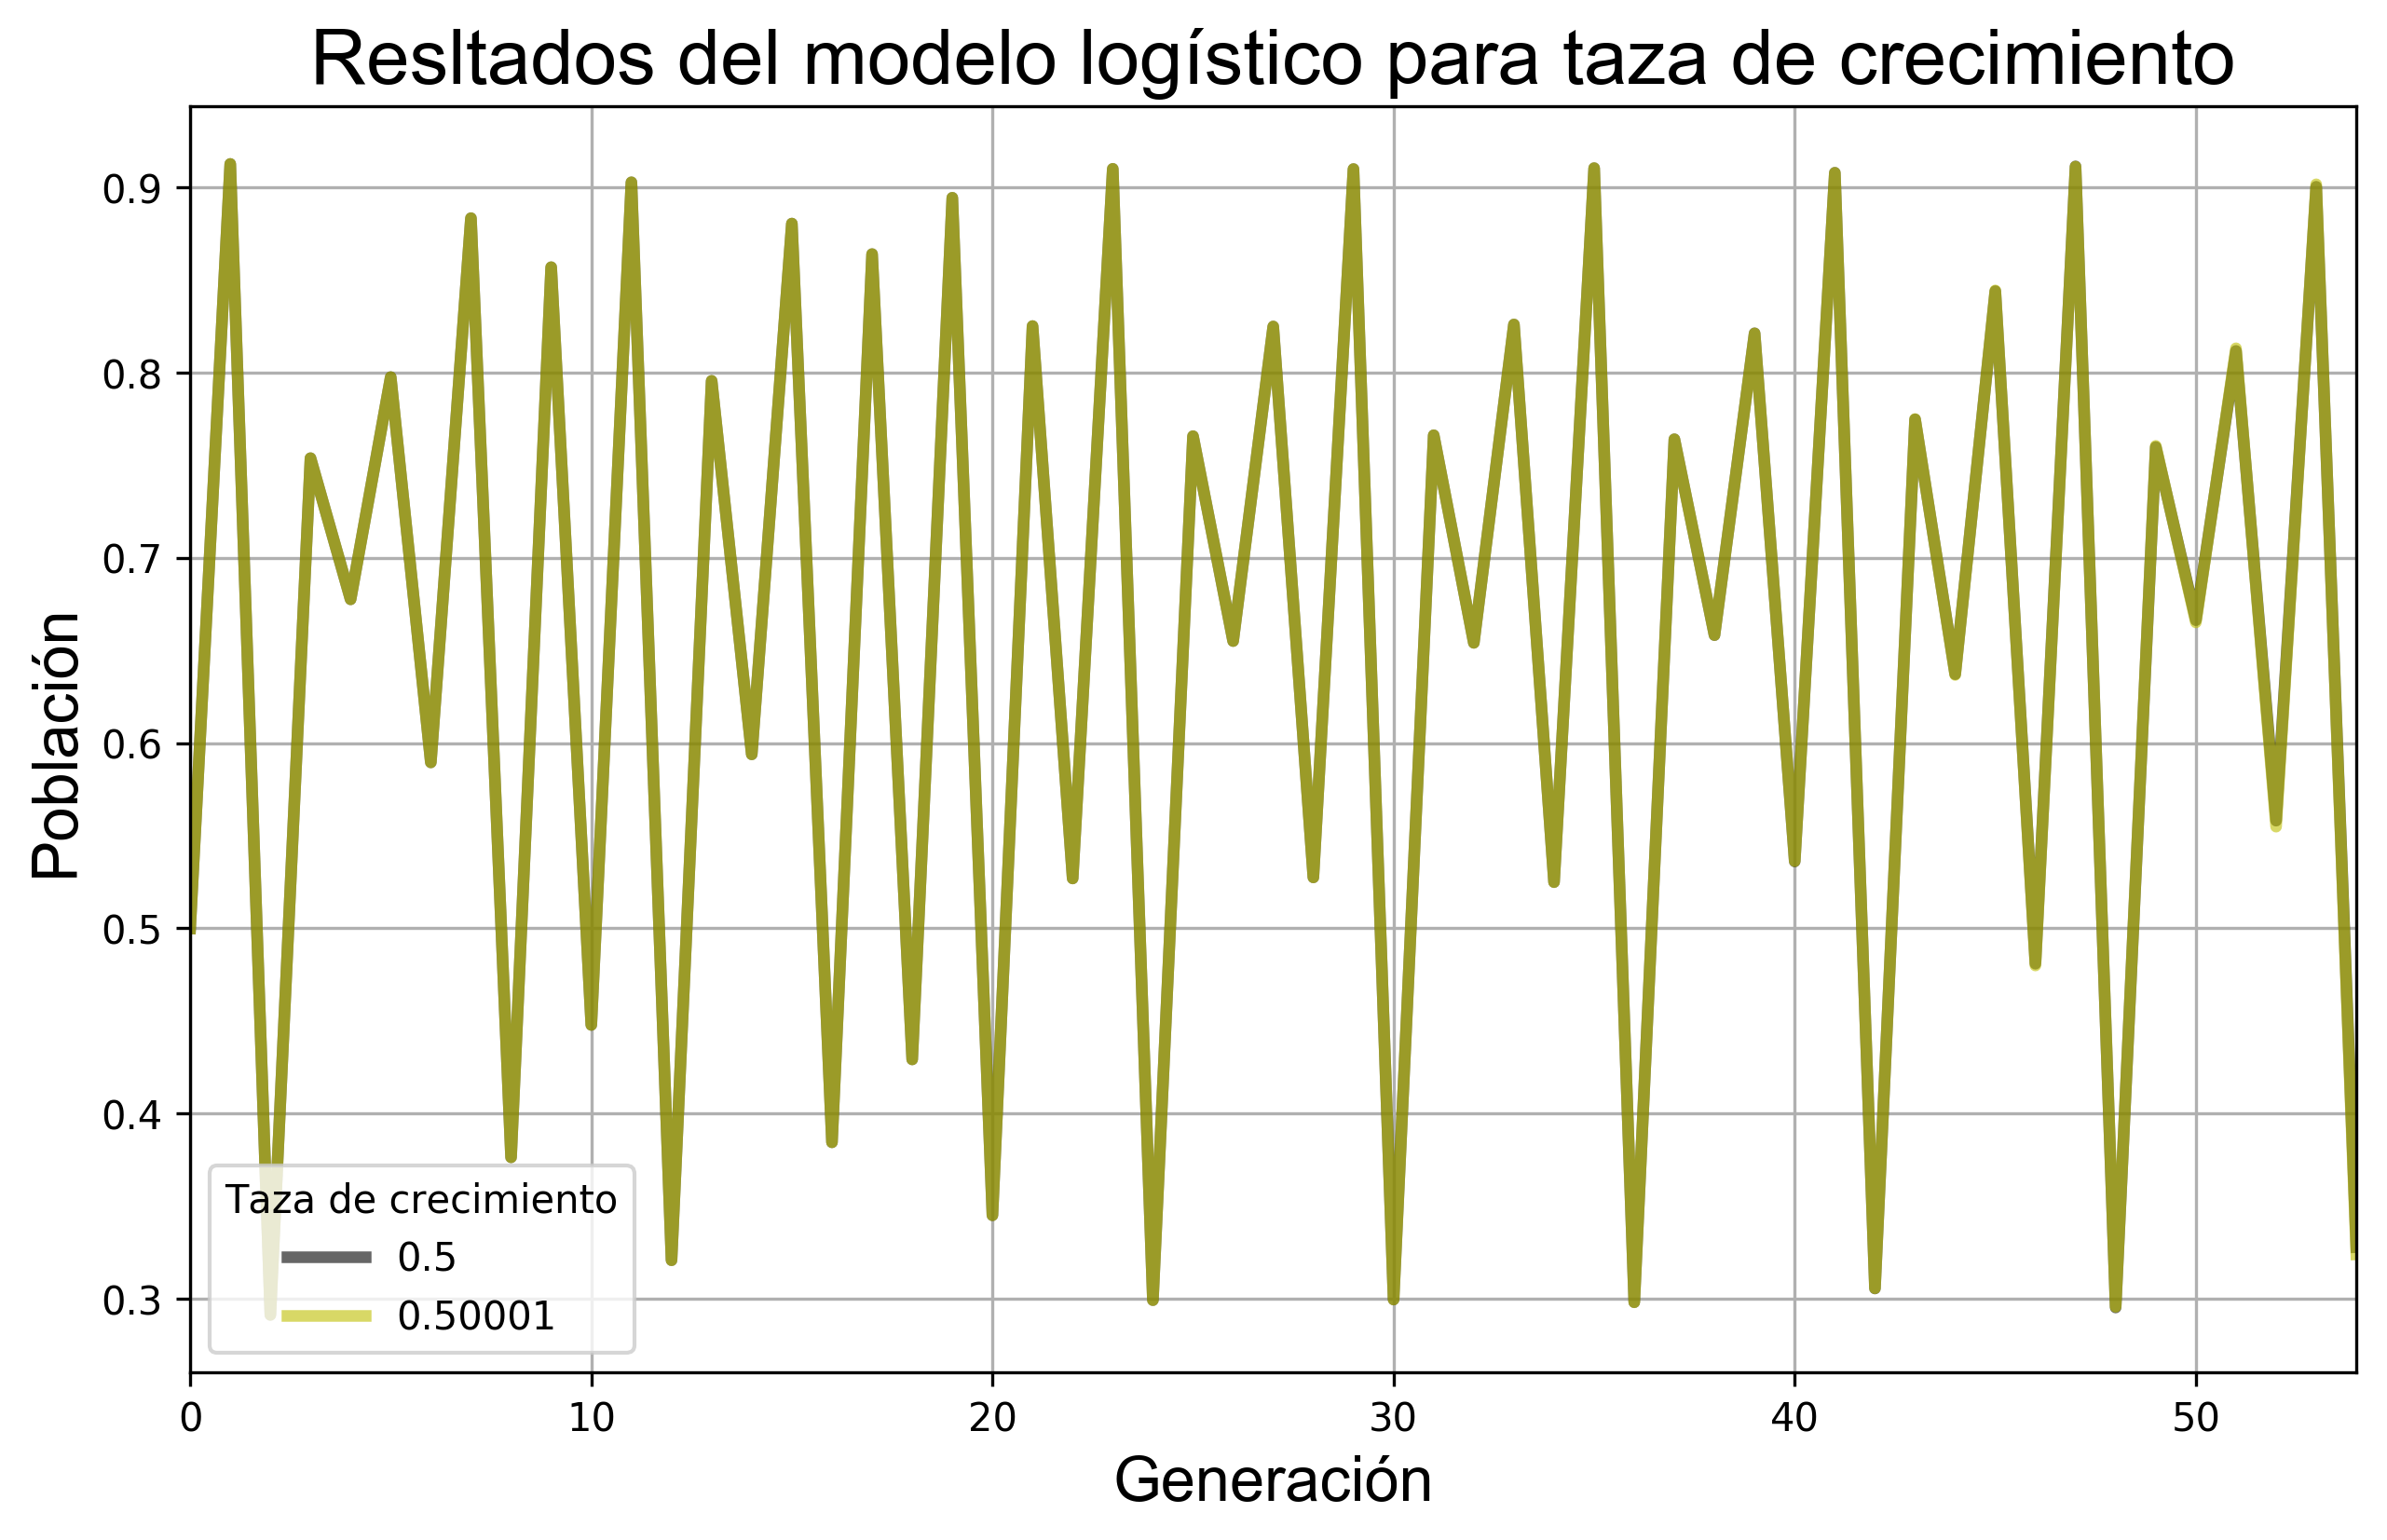
\includegraphics[scale=0.60]{logistic-map-initial-conditions-stable.png}
\end{center}


\textbf{\section{\LARGE Otros sistemas}}
Los que se presentan a continuación muestrán los atractores que influyen dentro de la población y sus tazas de crecimiento.

\begin{center}
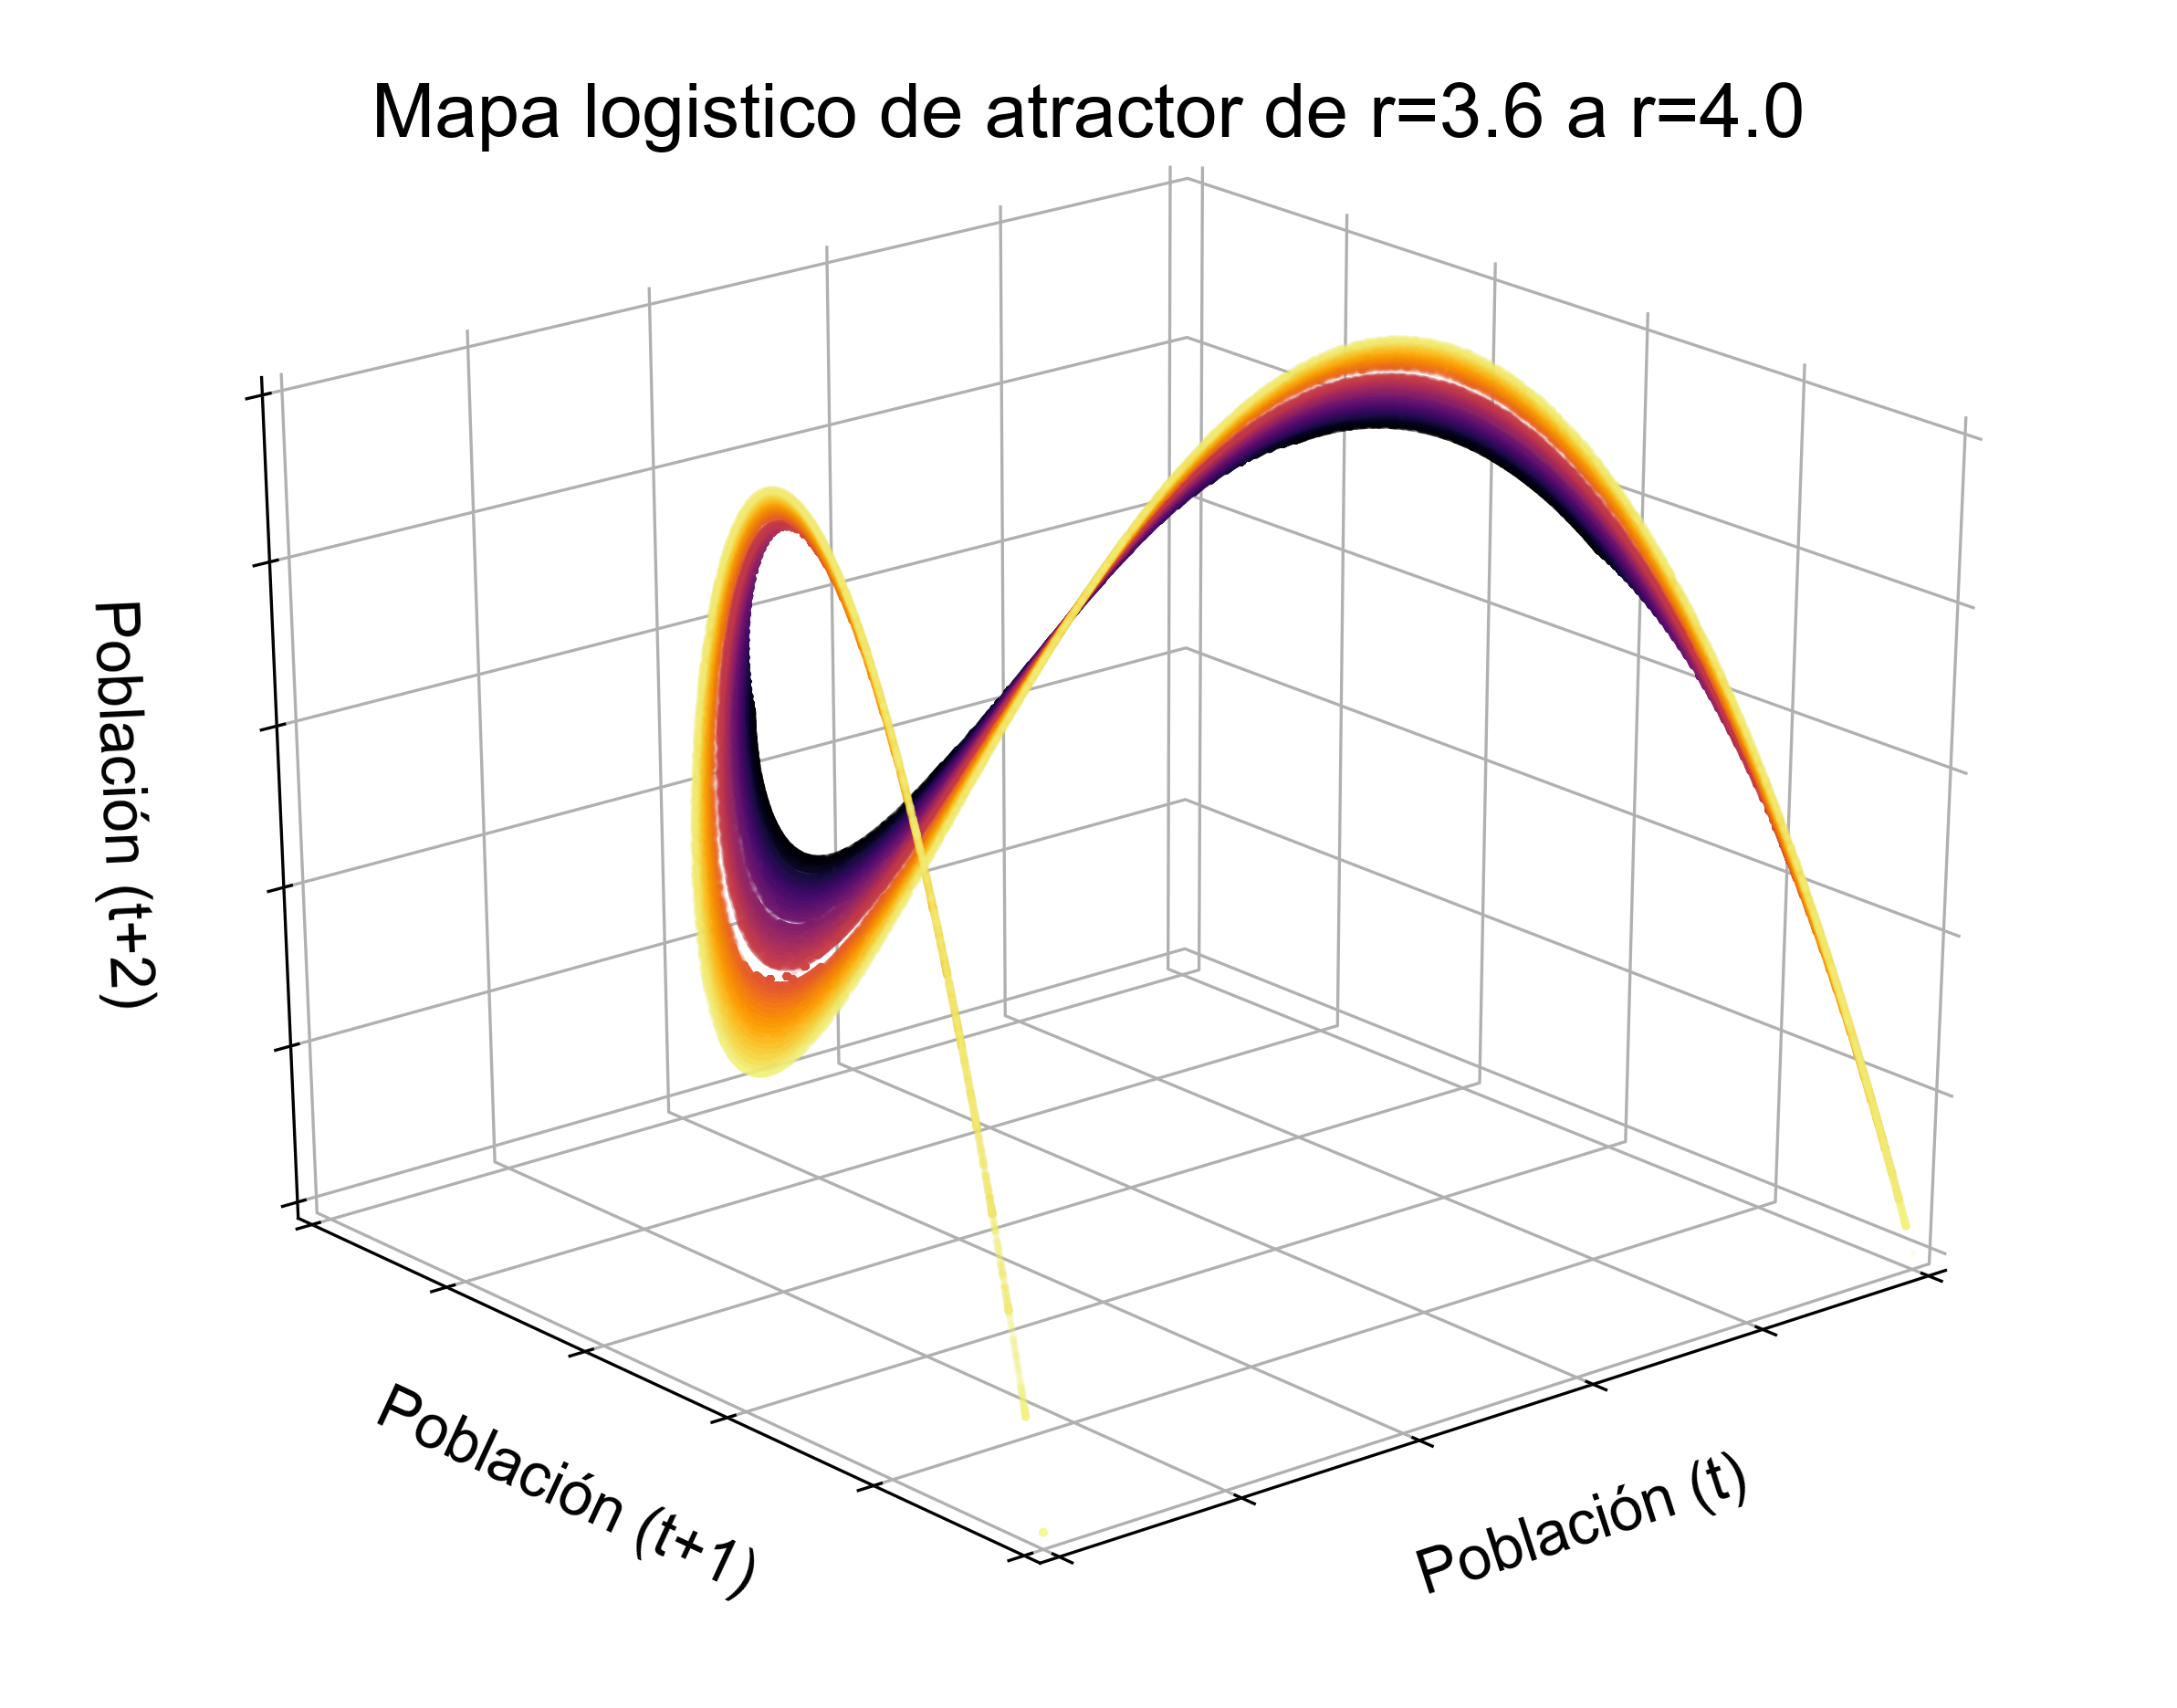
\includegraphics[scale=0.50]{3d-logistic-map-attractor-1.png}
\end{center}

\vspace{0.1cm}

\begin{center}
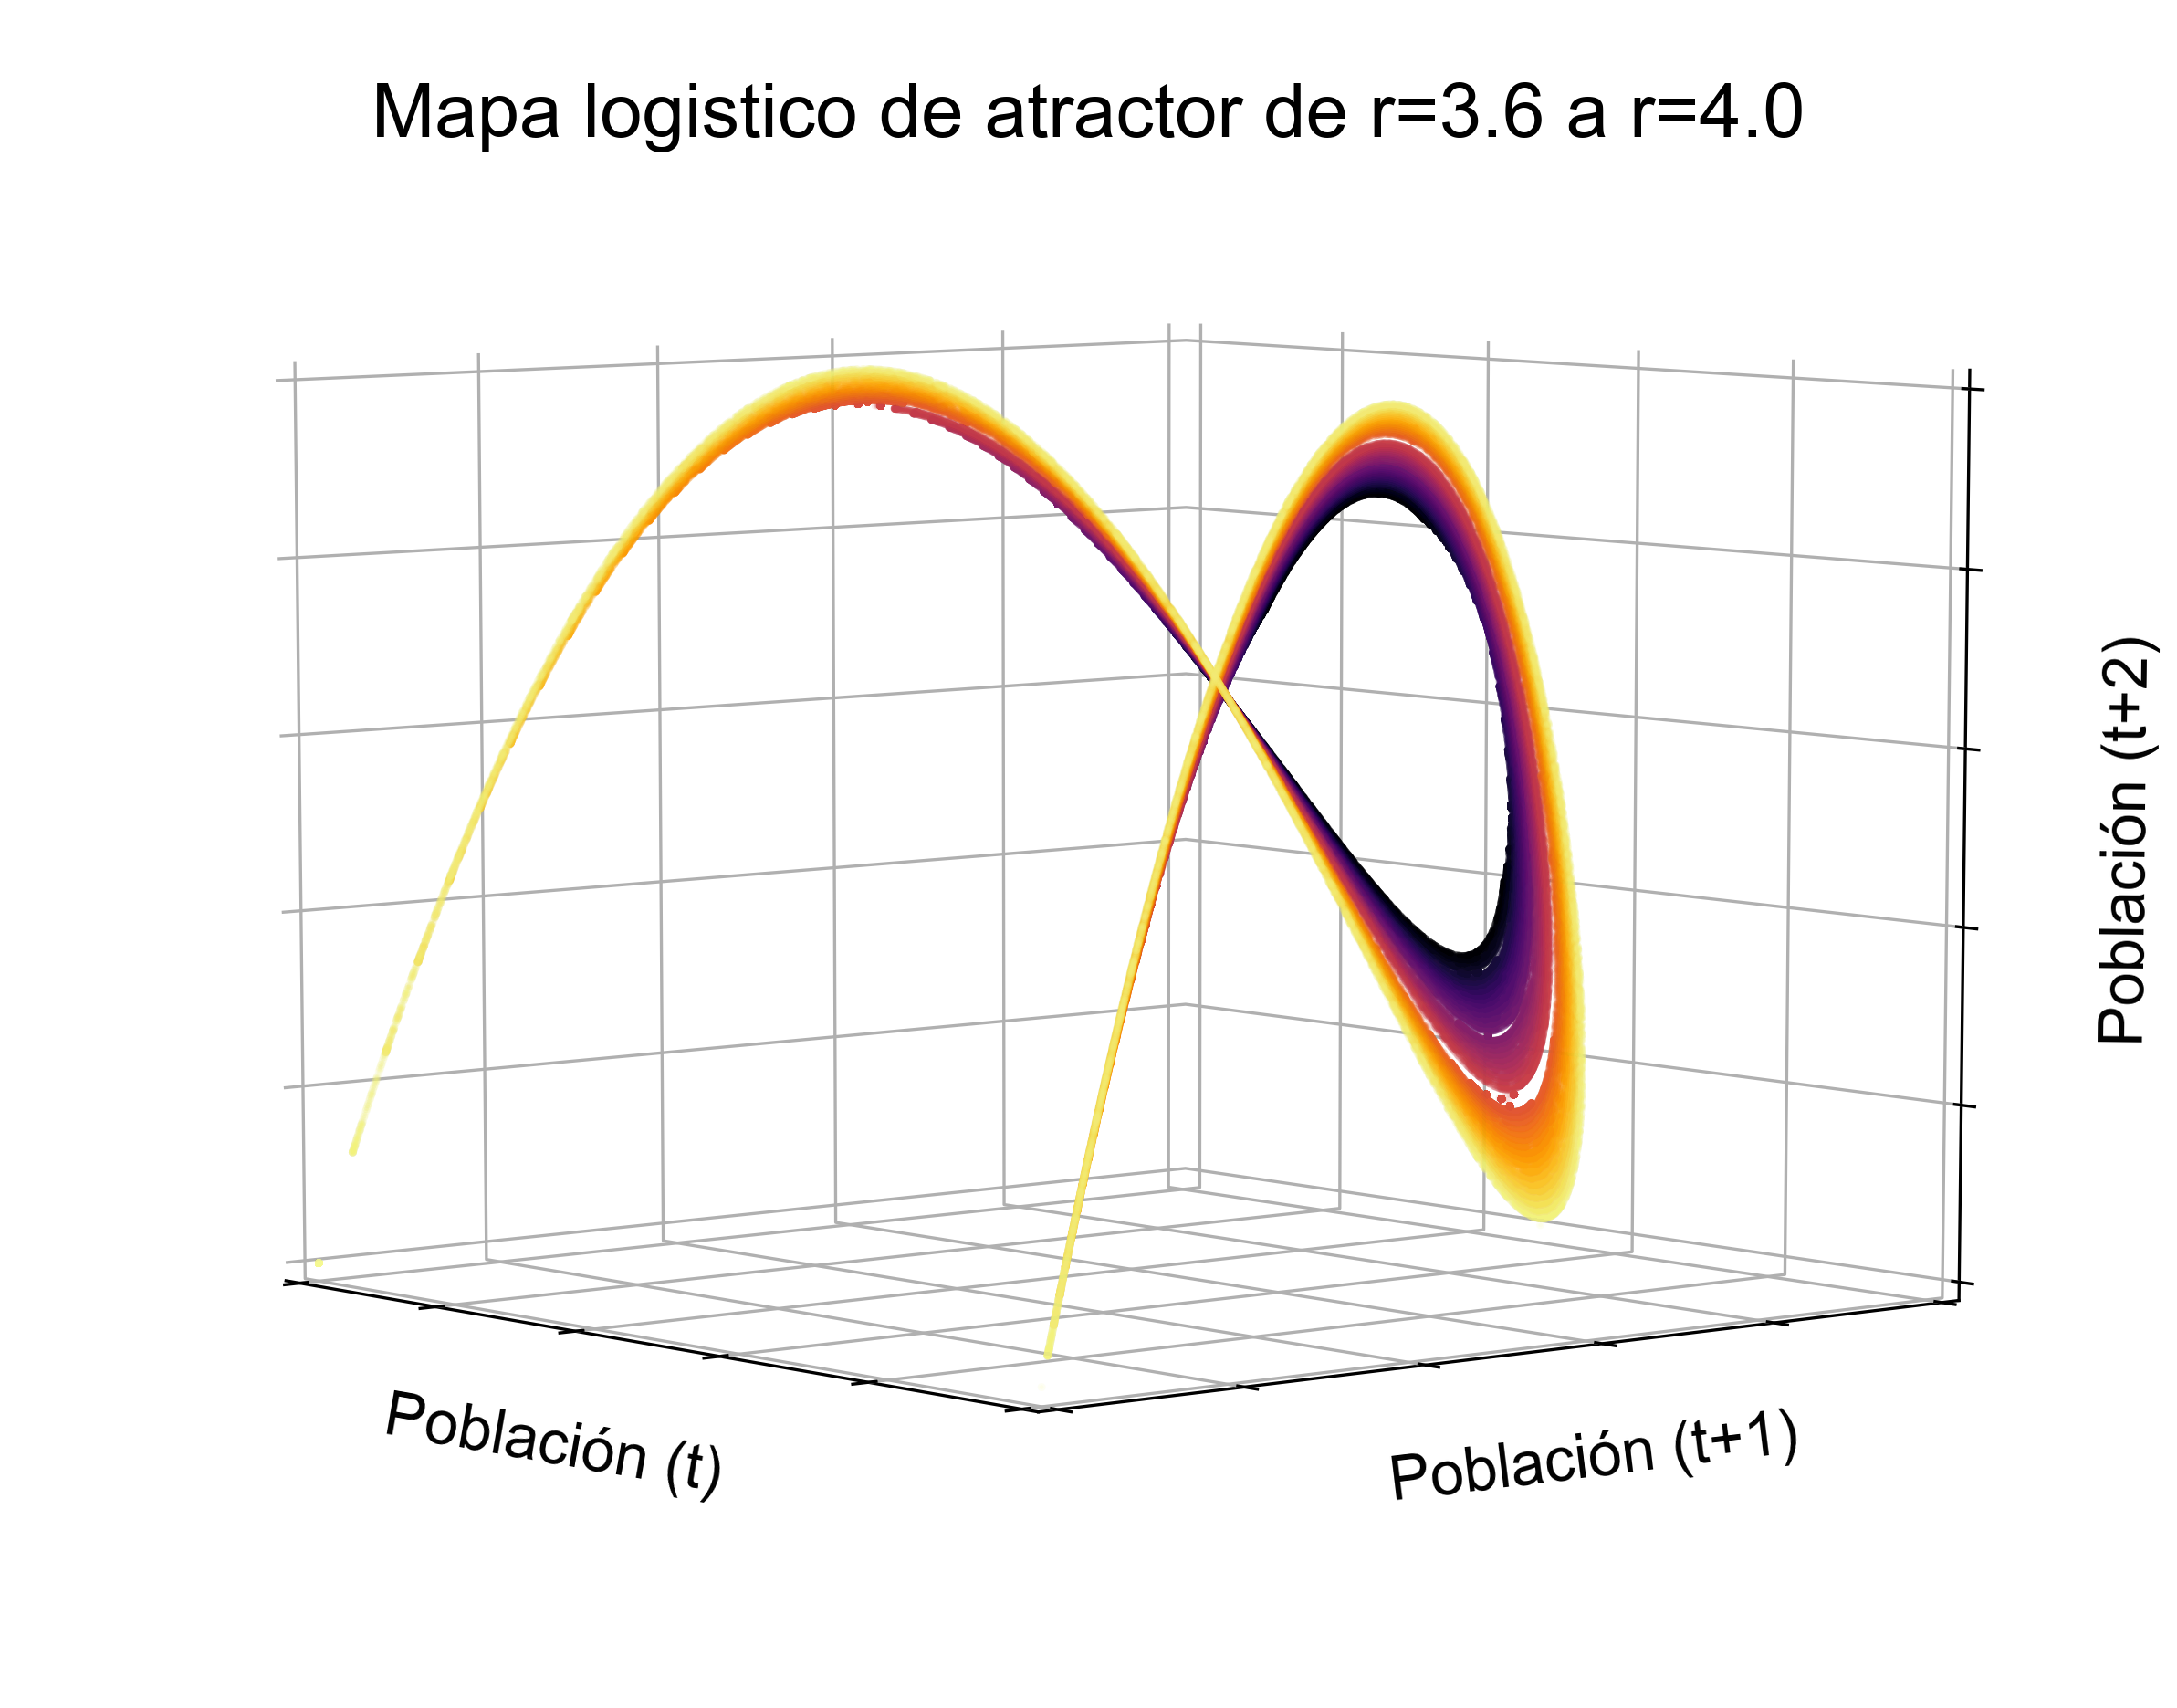
\includegraphics[scale=0.50]{3d-logistic-map-attractor-2.png}
\end{center}

\pagebreak

\textbf{\section{\LARGE Bibliografía}}

\begin{verbatim}
Recurrence relation. (2017). En.wikipedia.org. Retrieved 16 May 2017, 
from https://en.wikipedia.org/wiki/Recurrence_relation
\end{verbatim}

\end{document}